%
%
%
%%%%%%%%%%%%%%%%%%%%%%%%%%%%%%%%%%%%%%%%%%%%%%%%%%%%%%%%%%%%
\documentclass[a4paper, 11pt]{report}%choice of the class of the document
\usepackage[english]{babel}%choice of language
\usepackage{amssymb,bm,graphicx,graphics,subfigure,geometry}%different packages
\usepackage[breaklinks]{hyperref}
\usepackage[final]{pdfpages}%insertion of pdf
\usepackage{url}%format adress url
\usepackage{fancyhdr}% header and footer can be modified
\usepackage[official]{eurosym}% symbol of money euro. for dollar tape : \$
\usepackage{textcomp}%special letter
\usepackage{parskip}% for paragraph and skip
\usepackage[version=3]{mhchem}% for chemistry
\parskip=0.1in% for chemistry
\usepackage[italic]{hepnames} % for proton etc 
\usepackage{mathtools} % for math symbol
\usepackage{amssymb,amsmath}% for insert math eq in latex
\usepackage{hyperref} % for appendix and label
\usepackage{hyperref} % for appendix and label
\usepackage{qtree} % to create trees
\usepackage{color} % color the text

\newgeometry{top=3cm,right=2cm,left=3cm,bottom=3cm}

%%%%%%%%%%%%%%%%%%%%%%%%%%%%%%%%%%%%%%%%%%%%%%%%%%%%%%%%%%%%
%     few commandes to control geometry of paper :         %
% https://www.sharelatex.com/learn/Page_size_and_margins   %
%%%%%%%%%%%%%%%%%%%%%%%%%%%%%%%%%%%%%%%%%%%%%%%%%%%%%%%%%%%%

%\usepackage[a4paper, top=25mm, bottom=2mm, left=25mm, right=15mm]{geometry}
%\sloppy
%\addtolength{\headheight}{-2.0cm}
%\addtolength{\textheight}{+2.0cm}
%\addtolength{\oddsidemargin}{-0.5cm}
%\addtolength{\textwidth}{+1.0cm}

\setlength{\parindent}{15pt}%set alinea of paragraph. Default 15 pt. 

%%%%%%%%%%%%%%%%%%%%%%%%%%%%%%%%%%%%%%%%%%%%%%%%%%%%%%%%%%%%
% few commandes to have a quick acess for long expressions %
%%%%%%%%%%%%%%%%%%%%%%%%%%%%%%%%%%%%%%%%%%%%%%%%%%%%%%%%%%%%

%few commandes to have a quick acess for long expressFor the MPPC readout circuit, a current-to-voltage amplifi er can
\newcommand{\TPS}{T\'él\'écom Physique Strasbourg}
\newcommand{\PLG}{Paul LOPES GOMES }
\newcommand{\IR}{Internship Report}
\newcommand{\TotI}{Photo-detector development for nEXO}
\newcommand{\xfl}{Xenon flash lamp }
%for reference 
\newcommand*{\fullref}[1]{\hyperref[{#1}]{\autoref*{#1} \nameref*{#1}}} % One single link

\begin{document}

%%%%%%%%%%%%%%%%%%%%%%%%%%%%%%%%%%%%%%%%%%%%%%%%%%%%%%%%%%%%
%                     cover page                           %
%%%%%%%%%%%%%%%%%%%%%%%%%%%%%%%%%%%%%%%%%%%%%%%%%%%%%%%%%%%%

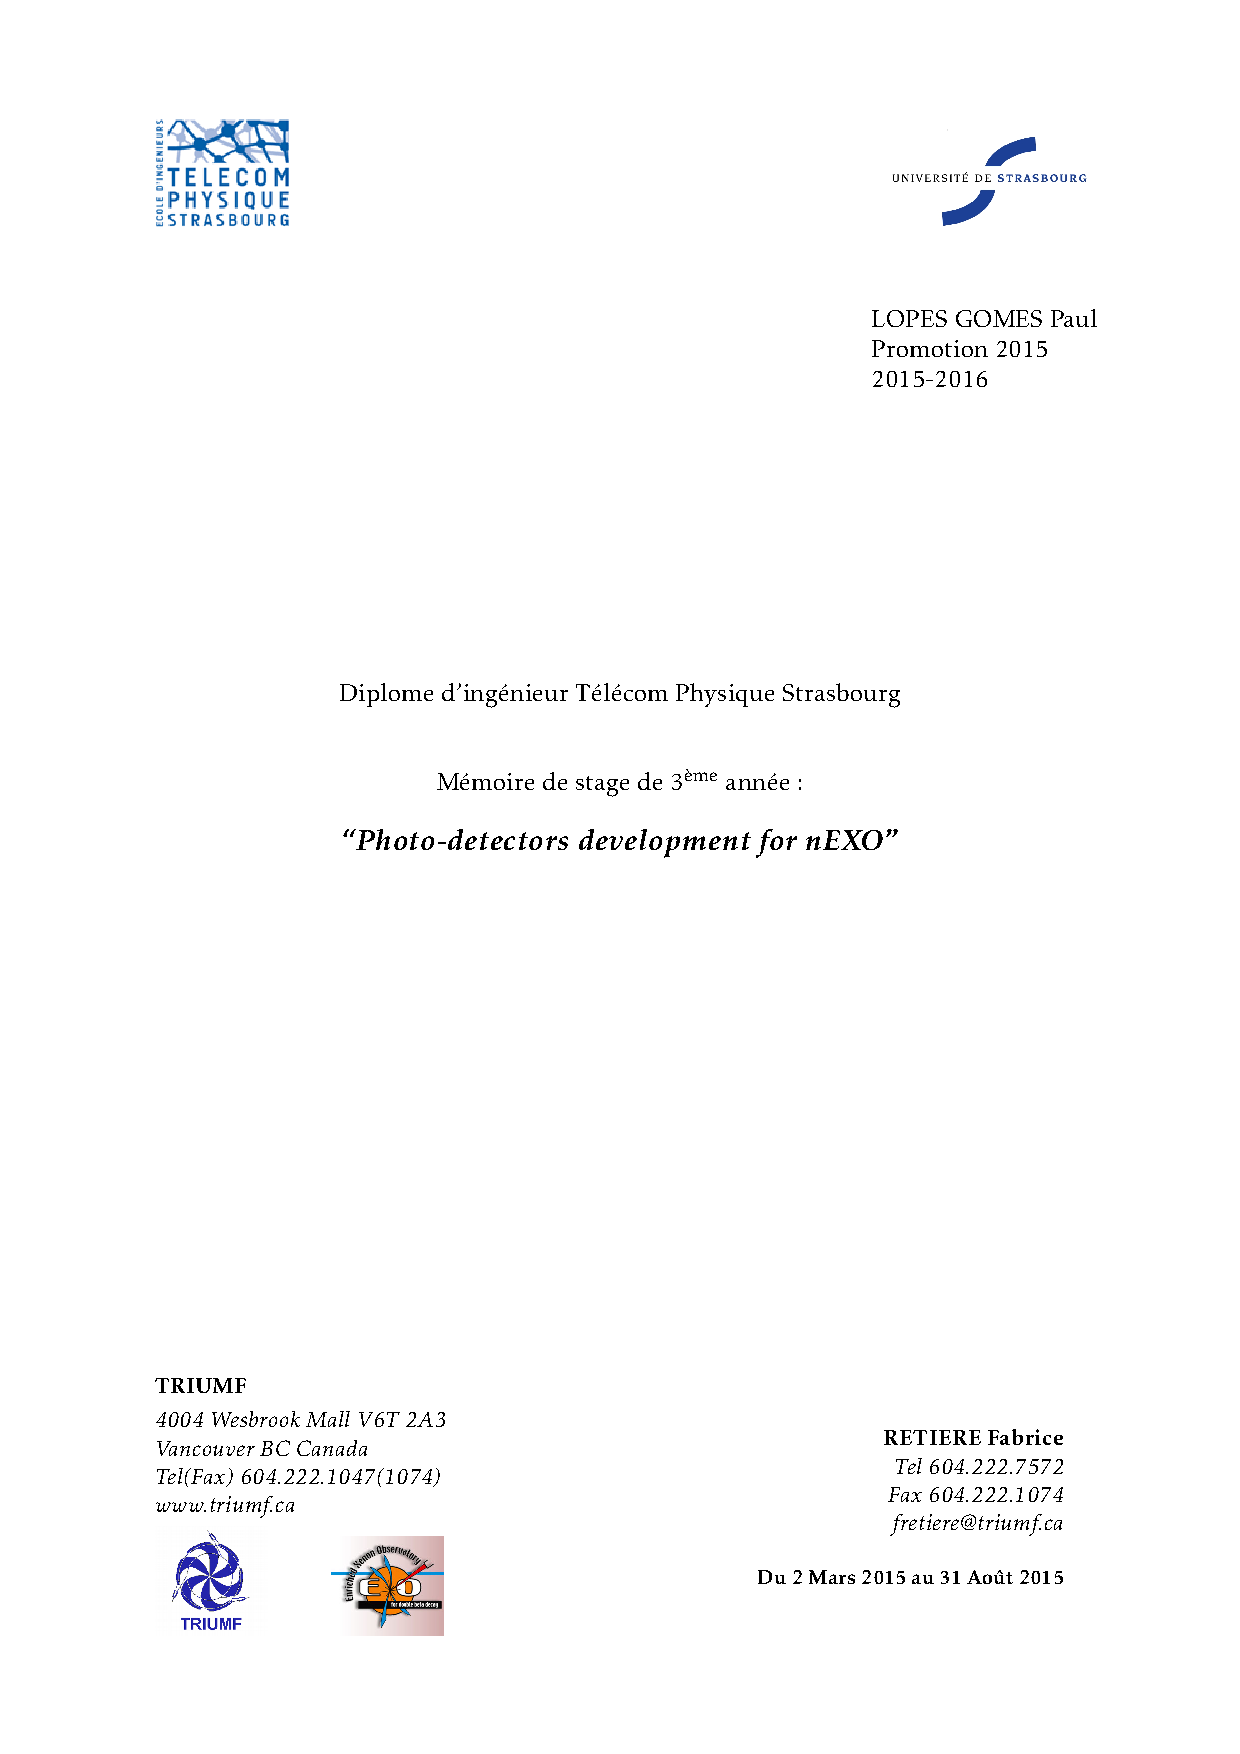
\includepdf{cover_page_TPS.pdf}

%%%%%%%%%%%%%%%%%%%%%%%%%%%%%%%%%%%%%%%%%%%%%%%%%%%%%%%%%%%%
%              a page to say thank you                     %
%%%%%%%%%%%%%%%%%%%%%%%%%%%%%%%%%%%%%%%%%%%%%%%%%%%%%%%%%%%%

\newpage
\thispagestyle{empty}

\vspace{1cm}
\paragraph{Thanks.}\hspace{1cm}
  
  Fisrt I would like to express my gratitude towards TRIUMF, a national laboratory for particle and nulcear physics, for having welcomed 
  me for those past 25 weeks of internship. I would lile to thank especially Mr. Fabrice RETIERE who supervised the work of my team. 
  \\ 
  
  Many thanks to Ms M. MCKAY who helped me to come in Canda/to obtain documentations required to go to Canda and who guided me towards 
  TRIUMF during my first days.
  Many thanks for Mr. P. Lu, Mr. C. CHAMPMAN et Mr. C LIM for their technical advises for this project
  \\
  
  I would like to thank in general each person who contributed that this intership became a real/ whole academical, prefesionnal and 
  humanly succeed. 
  / made this internship succeed/. Many thanks towards my co-workers : Ms. E. TONITA, Mr. C. RETHMEIER and Mr. L. JAMES. I thank also 
  some students from Ottawa's Unniversity : Jaqueline, Chriss and Mathiew.
  \\
  
  Finally I thank Ms. A.S. CORDAN, Mr. S. LECLER and Mr. J. BAUDOT for their advices and their from the beginning of my internship until my 
  defence for university . pour leurs conseils et leur suivis, 
  des premières démarches de mon stage jusqu'à ma soutenance pour le master PSA.
  \\

%%%%%%%%%%%%%%%%%%%%%%%%%%%%%%%%%%%%%%%%%%%%%%%%%%%%%%%%%%%%
%                        Abstract                          %
%%%%%%%%%%%%%%%%%%%%%%%%%%%%%%%%%%%%%z%%%%%%%%%%%%%%%%%%%%%%%

\newpage
\thispagestyle{empty}

\paragraph{Abstract}\hspace{0.5cm}\\
  
  Founded in 1968 and located on the campus of UBC \footnote{University of British Columbia}, TRIUMF \footnote{Canada's national laboratory 
  for particle and nuclear physics} is one of the world’s leading subatomic physics laboratories. Different research experiments in particle physics
  are conducted. On the microscopic scale TRIUMF and nEXO \footnote{next generation Enriched Xenon Observatory} work together to measure 
  the neutrino-less double beta decay. 
  \\
  \ce{^{136}Xe} may produce such decay, emitting light at 175 nm. My internship focuses on the characterisation of Silicum Photo-Multipliers which will be 
  used to detect this light in the nEXO experiment. To characterize them, efficiency dark noise and cross-talk were calculated
  at different over-voltages. Each SiPM has its own breakdown voltage beyond photons could be detected. 
  \\
  We characterized both MEG MPPC \footnote{SiPMs produced by Hammamatsu} and VUV3 SiPM at $-100^\circ$C. With an overvoltage of 3.5V for the MEG MPPC (breakdown 
  voltage of 57V at such temperature) and 11V (breakdown voltage of 44.7V at such temperature), the efficiency, the dark noise and the crosstalk were plotted. 

\paragraph{R\'esum\'e}\hspace{0.5cm}\\
   
   Fond\'ee en 1968 et localis\'e sur le campus de l'UBC, TRIUMF -Laboratoire national Canadien pour la recherche en physique nucl\'eaire et en physique des 
   particules- est l'un des plus importants laboratoires de physique subatomique au monde. Diff\'erents th\`emes de recherche dont celui des particles 
   sont envisag\'e. A l'\'echelle nanom\'etrique TRIUMF et nEXO travaillent ensemble \`a la recherche de la d\'esint\'egration bêta sans émission
   de neutrinos. 
   \\
   Si l'\'el\'ement chimique \ce{^{136}Xe} est un candidat potentiel pour produire une telle d\'esint\'egration avec \'emission de lumi\`ere \`a 175 nm, le but de mon 
   stage est de caract\'eriser des d\'etecteurs SiPM. De tels d\'etecteurs seront ensuite utilis\'es lors de l'exp\'erience nEXO pour d\'etecter la lumi\`ere
   (photons) \'emise. Ainsi il est possible de les caract\'eriser en calculant l'efficacit\'e, le bruit noire et le crosstalk à diff\'erentes tensions de polarisation. 
   Chaque SiPM a sa propre tension à partir de laquelle un photon est d\'etect\'e. 
   \\
   Le MEG MPPC ansi que le VUV3 SiPm ont \'et\'e caract\'eris\'e \`a $-100^\circ$C. Avec une suretension de 3.5V pour le MEG MPPC (La tension de rupture est 
   de 57V à cette temp\'erature) et de 11V pour le VUV3 SiPM (tension de rupture est de 44.7V), l'efficacit\'e, le bruit noire et le crosstalk ont \'et\'e
   trac\'es. 
   
%%%%%%%%%%%%%%%%%%%%%%%%%%%%%%%%%%%%%%%%%%%%%%%%%%%%%%%%%%%%
%                     contents page                        %
%%%%%%%%%%%%%%%%%%%%%%%%%%%%%%%%%%%%%%%%%%%%%%%%%%%%%%%%%%%%

\thispagestyle{empty}
\tableofcontents 



%%%%%%%%%%%%%%%%%%%%%%%%%%%%%%%%%%%%%%%%%%%%%%%%%%%%%%%%%%%%
%                     figures page                         %
%%%%%%%%%%%%%%%%%%%%%%%%%%%%%%%%%%%%%%%%%%%%%%%%%%%%%%%%%%%%

\thispagestyle{empty}
\listoffigures

%%%%%%%%%%%%%%%%%%%%%%%%%%%%%%%%%%%%%%%%%%%%%%%%%%%%%%%%%%%%
%                chapter 1 Introduction                    %
%%%%%%%%%%%%%%%%%%%%%%%%%%%%%%%%%%%%%%%%%%%%%%%%%%%%%%%%%%%%


\chapter{Introduction.}

  This internship of 25 weeks is the last session of teaching that \TPS offers to its students to complete/finalize their 
  engeneer studies. During this internship, the student should be able to realize/conduct a real engeneer or research work/The goal of this internship for the student is to show his 
  capability/able to/ to realize an real engeneer or research 
  work. 
  He's also asked to manage a project, to take its responsabilities and to show autonomus. 
  \\

  The subject of this internship covers the two main parts of teaching of \TPS. In fact I was asked to have some knowledges both in electronics, 
  waveform processing or cording and also in particle physics and matter physics. This last part/ had been taught by the master of Subatomics Physics
  and Astrophysical 
  
  This report will describe first of all the laboratory TRIUMF and the project on which I worked. Then I will ...
  At least I will conlcude. 
  \\
  
  Some appendixes will give more details of my work /the reader could find any appendix to go deeper in understanding of the subject.
  

%%%%%%%%%%%%%%%%%%%%%%%%%%%%%%%%%%%%%%%%%%%%%%%%%%%%%%%%%%%%
%        chapter 2 a short abstract about TRIUMF   3 pages    %
%%%%%%%%%%%%%%%%%%%%%%%%%%%%%%%%%%%%%%%%%%%%%%%%%%%%%%%%%%%%

\chapter{A short abtstract about TRIUMF}


  \section{History and Partners}

  \subsection{History}

  I worked at TRIUMF from the beginning of April 2015 to the end of August 2015.
  \\
  
  TRIUMF is one of the world’s leading subatomic physics laboratories and is considered Canada's leading nuclear science research institute. 
  Founded was founded in 1968 by a consrotium of four university whose the University of British Columbia.The goal was to provide a research 
  need in particle physicis. This laboratory is located on the campus of the University of British Columbia since 1971. It was built around 
  a cylcotron and the first beam of particles was produced in 1974.
  
  \begin{figure}[!hbtp]
  \centering
  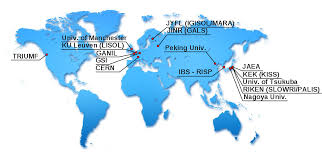
\includegraphics[trim=1.5cm 2cm 5.5cm 3cm, clip=true,totalheight=.4\textwidth]{../Pictures/TRIUMF_localisation.jpg}%trim=10cm 4cm 1cm 12cm, clip=true, 
  \caption{TRIUMF on the  globe.}
  \label{fig:TRIUMF_localisation}
  \end{figure}
  
  Over the year four main steps reflect researches conduct at TRIUMF and since 2009 TRIUMF is available to conduct research in different domains: 
  accelerator facility for nuclear, particle, medical and material science. 
  
  \subsection{Parteners}
  
  As no single university could provide research needs, 19 different member and associative unversities from across Canada belong to a consertium
  which/that governs TRIUMF// As no single university could provide research needs, the initial consertium enlarges up to 19 different 
  member and associate member universities from across Canada. This consortium rules TRIUMF and has allowed it to evolve into a national 
  laboratory. while still maintaining strong ties to the research programms of the CAnadian universities. 
  \\
  
  TRIUMF provides the centralized resources, tools, and expertise for its different Canadian parternship. These parternships could be 
  brought together in three different group/class: 
  \begin{itemize}
  \item Canadian unversities parteners,  
  \item Internional parteners,   
  \item Driving innovation with commercial partners. 
  \end{itemize}
  
  \section{Governance and Organisation}
  
  Even if TRIUMF is laboratory, it could be considered like an enterprise that includes on-site technical, engineering and administrative
  staff. Here is the origin of people in TRIUMF (Draw a circle with university researchers and students). 
  
  %private-sector collaborators and licensees; international collaborators; and publicly funded agencies supporting basic research 
  %in Canada’s interests. TRIUMF’s organization reflects these multiple stakeholders working together in concert.
  TRIUMF is a mix of resources  which let it to live in autoartsie. All piece for our porject was designed and made at TRIUMF. 
  \\
  
  %The mix of resources at TRIUMF is very different than at a university. This results in different synergies than are possible at a 
  %university. In fact, TRIUMF’s main strength is that it has a range of resources, both human and hardware, that can be applied coherently 
  %to a given problem. A typical TRIUMF user from the Canadian research community obtains technical support, collaborates with on-staff 
  %scientists, and may use a TRIUMF project engineer. This is in addition to any use of the physical resources. University-based 
  %researchers want to work with TRIUMF because these resources simply are not available at their home institutions. 
  %Scientists at TRIUMF become the key points of contact for their research. This contact helps foster collaborative partnerships among 
  %Canadian researchers and between Canadian researchers and their international colleagues. TRIUMF also provides salary support 
  %(in whole or in part) for about a dozen scientists resident at Canadian universities. This support strengthens the scientific and 
  %intellectual ties between TRIUMF and the universities. In addition, as an active research centre, TRIUMF maintains an atmosphere 
  %that promotes intellectual activity through seminars, visitor programs, and workshops. Tying it all together is a management structure 
  %geared to maximizing the science impact for Canada.
  
  TRIUMF is organized to optimally meet its objectives while maintaining accountability, quality, and effectiveness. That is why this laboratory is divided
  in eight different divisions :
  
  \paragraph{\underline{\emph{Science Division}}}
    
  I belonged/worked in the Science Division. Physical Sciences  is responsible for scheduling experiments approved by the 
  Experimental Evaluation Committee (EEC). This division is also responsible for all components of all systems and subsystems both for all 
  experimental operations at the TRIUMF site and for other infrastructure for external programs whose nEXO. 
  \\
  
  Here is the organigram : 
  
 % {\qtreeshowframes
 % {\Tree 
 %   [.Head of TRIUMF: \textit{\textcolor{blue}{Dr. Jonathan BAGGER} } 
 %     [.Head of Science Division: \textit{Dr. Reiner KRUECKEN} %
%	[.Head of Science technology: \textit{Dr. Fabrice RETIERE} 
%	  [.Head of Developement: \textit{Dr. Fabrice RETIERE} 
%	  [.Developement of photo-detectors for nEXO: \textit{Dr. Fabrice RETIERE} {Carl RETHMEIER} {Llyod JAMES} {Paul LOPES GOMES} !{\qbalance}] %last !{\qbalance} 
%	  ] 
%	] 
 %     ]	
  %  ] 
 % }
  
  
  \section{Research topics at TRIUMF}
  
  As a publicly-funded national laboratory, TRIUMF's activities are framed within its mission and vision with a strategic plan developed 
  every five years and subject to review, approval, and funding by the Government of Canada and other agencies.\\
  The strategic plan of TRIUMF could be divided in three main parts : 
  \begin{itemize}
  \item The advancing isotopes for science and medicine,  
  \item The harnessing particles and beams for discovery and innovation,   
  \item The understanding of the building blocks od matter and how they shape our universe. 
  \end{itemize}

  Seven different research topics are conducted at TRIUMF, from some research in nulcear medicine to the investigations in theory group 
  through the particle physics. 
  \\
  
  Ultimately, these programs are based on pure research in subatomic physics 
  and exploit the opportunities provided by TRIUMF’s core facilities and its synergy with the university research community.\\
  The driving motivation behind particle physics experiments is the desire to uncover the true nature of fundamental forces and particles. 
  Our current standard model \footnote{ad ref to publication or book} believed to be an effective theory, which has a deeper underlying theory reachable in the next generation 
  of experiments. 
  \\
  For exemple in particle physics, in the electroweak sector \footnote{ref to publication or book}, where great successes of the past decades have predicted and verified the unification of the 
  electromagnetic and weak nuclear forces, precision measurements at the CERN large electron positron collider (LEP) and the Fermilab 
  proton-antiproton collider (Tevatron) demand that there be either a light Higgs particle with a mass less than about 200 GeV or a 
  physical system mimicking its interactions. 
  \\
  
    
%As it cores different research topics whose 
%SNOLAB’s ultra-low background places it centre stage in two quests: on the cosmic scale for interstellar dark matter and on the microscopic scale for neutrinoless double-beta decay. Astrophysical measurements indicate that 80% of the matter in the universe is “missing,” that is, we can see its gravitational effects but it does not emit any heat or light. This “dark matter” is hypothesized to be the stuff that shapes the destiny of the universe, and yet we have no idea what it really is.

%Experiments at SNOLAB will search for hypothesized rare interactions between dark matter and normal matter. On the microscopic end of the spectrum, neutrinoless double beta decay probes the very nature of antimatter. Advanced theories of particle physics and the Big Bang suggest that the neutrino particle may have a special nature: it might be its own antiparticle. Answering this question about the neutrino could reveal new insights into why the modern universe is predominantly occupied by matter (including dark matter!) rather than anti-matter.

%The initial program of SNOLAB will likely include experiments that focus on direct detection of dark matter (DEAP/CLEAN, PICASSO, Super-CDMS) and neutrinoless double-beta decay (SNO+, EXO).
  
  \paragraph{\underline{\emph{From SNOLAB to EXO}}}
  
  SNOLAB’s experiment places it centre stage in two quests on opposite scale : on the cosmic scale for interstellar dark matter and on the 
  microscopic scale for neutrinoless double-beta decay. 
  \\
  
  On the cosmic scale astrophysical measurements indicate that $80\%$ of the matter in the universe is ``missing'', which means
  that this matter does not emit any heat or light. This matter is called dark matter.\\
  Experiments at SNOLAB will search for hypothesized rare interactions between dark matter and normal matter. On the microscopic end of 
  the spectrum, neutrinoless double beta decay probes the very nature of antimatter. 
  Advanced theories of particle physics and the Big Bang suggest that the neutrino particle may have a special nature: it might be its own antiparticle. 
  Answering this question about the neutrino could give light/explain/guided research on the cosmics scale. 
  \\
  
  So initial programs of SNOLAB include bisaclly/likely experiments that focus on direct detection of dark matter (DEAP/CLEAN, PICASSO, 
  Super-CDMS) on the cosmic sacle and also on direct detection of neutrinoless double-beta decay (SNO+, EXO) on the microscpic scale. 
   
  
  
%%%%%%%%%%%%%%%%%%%%%%%%%%%%%%%%%%%%%%%%%%%%%%%%%%%%%%%%%%%%
%          chapter 3 presentation fo the subject 4/5 pages       %
%%%%%%%%%%%%%%%%%%%%%%%%%%%%%%%%%%%%%%%%%%%%%%%%%%%%%%%%%%%%

\chapter{nEXO's experiment} % the neutrino and the nEXO experiment
 

  \section{Understand physical phenomena}%The neutrino, a majorana particle ? % Physics behind the experiment % 
  
  Our don't let us see too small thing/to observe what are made matter/what matter is made. So it has been proved , theoritically and by experiment that matter is made of (number)of particle \footnote{quote ref book}. The most known elementary particle is electron which conduct current in 
  electrical installation for exemple. But it is quiet known that light has the properties of both a wave and a particle, called photon. 
  At least there is also
  neutrinos. Each of those particle have their physical propreties.
  \\
  
  On of the basic rule of the nature \footenote{ref book} is that when a particle is create, another opposite particle is creating on the same time : the lasts are 
  called anti-particle with their opposite properties. 
  
  (tableau des particle et antiparticle). 
  
  These particle consist the matter/ We are made of this particle/A ll matter (both humain or space) are made of this particle and as we are 
  continously roket by these particle, it is possible to to obsere/to quantify/to calculate the mass/to describe their physical properties 
  (mass, energy etc) by using different detector. (remain the main family of detector ? )
  \\
  
  \subsection{The neutrino a Majorana particle ?}
  
  As the array above could give some indication, neutrino is part of elementary particle.\\
  A currently quest about neutrino is to check if neutrino has a certain characteritics/properties which is to be a Majorana particle\ is 
  to determine properties of neutrino : Majorana particle, calculate the mass etc\\
  The double beta decay/reaction let us determine those characteritics. The Standard Model \footote{ref aout SM, or explication what it is}
  predicts the ordinary double beta decay \(2\Pneutrino\beta\beta\). 
  %The detection of \(0\Pneutrino\beta\beta\) would validate ``Physics beyond the standard model''\footnote{same}, show that the neutrino is a Majorana particle and give a measure of the absolute neutrino mass. 
  \\
  
  \ce{^{136}Xe} is one of the 35 natural isotopes capable of \(2\Pneutrino\beta\beta\). If \(0\Pneutrino\beta\beta\) is possible, 
  it would occur in \ce{^{136}Xe} according to this reaction : 
    
  \begin{equation}
    \ce{^{136}Xe} \rightarrow \ce{^{136}Ba} + 2\Pelectron %\iff 2\Pneutron \rightarrow 2\Pproton + 2\Pelectron \iff \ce{^{136}Xe} \rightarrow 2\APneutrino + 2\Pelectron 
  \end{equation}
   
  The two electrons, which are ejected with high kinetic energy, scatter off the electrons of other \ce{^{136}Xe} atoms. If so, one 
  of the impacted \ce{^{136}Xe} atoms is excited from the ground state and then de-energizes by releasing photons. 
  This is knowen as scintillation process. The wavelength of the created light is 175 nm. 
  \\
  %% presentation thesis
  
  Current limits on the half-life of \OB are > 10up(25) yr, providing a 
  formidable challenge. The Enriched Xenon Observatory (EXO) is a 
  double beta decay experiment poised to improve upon this limits, using
  xe136 as both a source and detector of this decay. \(0\Pneutrino\beta\beta\) of xe136 produces a detectable
  energy deposition....
  
  One possible method of measuring the neutrino mass is by observation of a rare, 
  as yet unseen, second order electroweak process called neutrinoless double 
  beta decay (\(0\Pneutrino\beta\beta\)). \\
  EXO is designed to search for thsi decay in xe136. In the standard version
  of this process (\(2\Pneutrino\beta\beta\)) a xe 136 decays to a ba136++, emitting two electrons and two anti-neutrinos. 
  This process has been observed in various nuclei, but doesnot allowfor a measuremetn
   of absolute neutrino mass. 
   
  
 beta decay is the simplest method of making an absolute neutrino mass measurement. 
 \(0\Pneutrino\beta\beta\) has the potential to probe mass limits in the meV range (combining cosmological and oscillation
 results, one neutrino mass should be in the range mvelec = (0.04-0.1) ev. Confirmation by 
 exo in ...), provided neutrinos are Majorana particles, ad lepton number
 conservation is violated. 
 \(0\Pneutrino\beta\beta\) is  due to the exchange of light Majorana neutrinos, the neutrino mass
 spectrum is strongly degenerate . 
 
 % double beta decay thesis
 
 Two neutrino double beta decay (\(2\Pneutrino\beta\beta\)) is a standard second-order electroweak
 process, whereby a nucleus with charge Z and mass number A decays to a nucleus
 with charge Z+2 and mass numberA, where both Z and A are even. We speak about even-even nuclei (like evn-odd nuclei or odd-odd nuclei). 
 
 \begin{equation} \label{eq:charge}
    (A,Z) \rightarrow (A,Z+2) + \Pelectron1 + \Pelectron2 + \APneutrino1 + \APneutrino2
 \end{equation}
 
 Z is the number of proton and A is the number of proton and neutron. As ``rien ne se pert, rien ne se cre, tout se transforme'', 
 the equation above means that in this process, 2 neutrons decay to 2 protons. 
 
 The array of section above and the conservation of the charge \footnote{rule in physics} 
 implies the creation of two electrons \ref{eq:charge}. \\
 
 As 2 electrons appear and according to the array above, the conservation of the leptonic electronic number \footnote{another rule} 
 implies the creation of two anti-neutrino \ref{eq:leptonic}:  
 \begin{equation} \label{eq:leptonic}
    0 \rightarrow 0 + 2*(+1) + 2*(-1)
 \end{equation}
  
 So the equation is right. 
 
 Now the total energy difference (which is difference between mass. Mass of particle are expressed in energy since einstein low
 direct relation/tie between mass and energy) between the initial and final nuclei
 is called the Q-value. In \(2\Pneutrino\beta\beta\), this energy is distributed among the emitted electrons, neutrinos, and nuclear 
 recoil of the daughter nucleus. As it has been said, this process occurs in various
 'even-even`` nuclei, with a certain rate. This rate would be dwarfed by the single 
 beta-decay rate, if it were not for a perculiarity in the nuclear mas function of certain
 even-even nuclei. This is shown for the case of xe136 in fig. number where single beta-decay to cs136 is energetically disfavored
 over \(2\Pneutrino\beta\beta\) to ba 136++. Possible  if the decay endpoint large enough which means Q>2 Mev). 
 
 This process is observed experimentally via the sum electron energy spectrum. 
 The electron energy spectrum of \(2\Pneutrino\beta\beta\) is continous, as the neutrino can be emitted with a kinetic
 energy between 0 and Q. 
 
 Complete it. 
 
 2 isotopes provides in particular a means of eliminating radioactive back-grounds. 
 \(0\Pneutrino\beta\beta\) of xe 136 produces 136 ba++(which become 136 ba+ by capturing an electron from the lXe conduction
 band) which can be identified via resonance fluorescence immadiately after the decay. The 
 EXO-200 and EXO experiements, described below, look for  \(0\Pneutrino\beta\beta\) using xe136. 
  
  %% other presentation
  To explain the \(0\Pneutrino\beta\beta\), lets start by reminding the double \(2\Pneutrino\beta\beta\) according the Standard Model. 
  As two neutrons become in two protons, the conservation of the charge implies the creation of two electrons \ref{eq:charge}. As 2 electrons appear, 
  the conservation of the leptonic electronic number implies the creation of two anti-neutrino \ref{eq:leptonic}:  
  
  \begin{equation} \label{eq:charge}
    (A,Z) \rightarrow (A,Z+2) + 2\Pelectron + 2\APneutrino
  \end{equation}
  leptonic electronic conservation :
  \begin{equation} \label{eq:leptonic}
    0 \rightarrow 0 + 2*(+1) + 2*(-1)
  \end{equation}
  
  Now lets consider the case when neutrinos are Majorana particles \footnote{ In opposition of Dirac particles where particles are distinct from anti-particles.}
  which means particles and anti-particles are identical except for their helicities. If so switching the helicity in this way allows 
  a particle in one frame of reference to be an anti-particle in another.
  \\
  That means that the emitted anti-neutrinos is neutrinos which conducts to the equation :
  
  \begin{equation}
    (A,Z) \rightarrow (A,Z+2) + 2\Pelectron + 2\Pneutrino
  \end{equation}
  
  Here we can observe the lepton number violation which would be an observation of ``Physics beyond the standard model'' :
  
  \begin{equation}
    0 \rightarrow 0 + 2*(+1) + 2*(+1)
  \end{equation}
  
  The Feyman diagrams related to \(2\Pneutrino\beta\beta\) and \(0\Pneutrino\beta\beta\) would be \cite{ref:beta_decay}: 
  
  \begin{figure}[!hbtp]
  \centering
  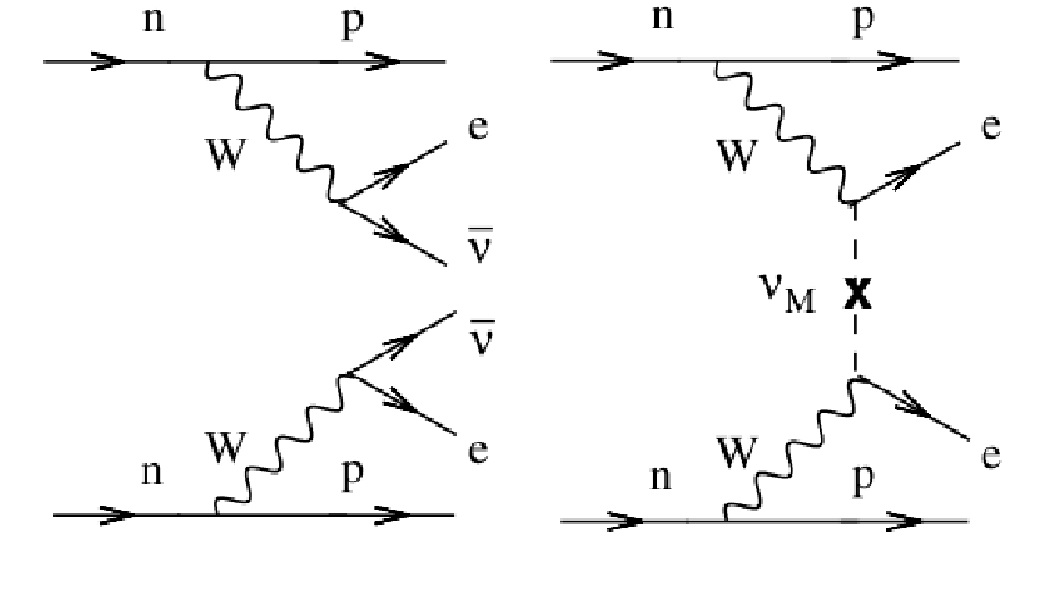
\includegraphics[totalheight=0.5\textwidth,trim=0cm 0cm 0cm 0cm, clip=true]{Pictures/blabla/beta.jpg}
  \centering{\caption{The \(2\Pneutrino\beta\beta\) (left) and the \(0\Pneutrino\beta\beta\) (right) : a virtual \Pneutrino instead of two \APneutrino.}
  \label{fig:feyman}
  \end{figure}
  
  
  Recent neutrino oscillation results provide experimental proof that neutrinos 
  are massive particles. These measurement, however, reveal information about 
  neutrino 
  
  \subsection{From EXO-200 to nEXO}
  
  The first phase of the EXo is a double beta decay experiment currently under construction, 
  employing 200 kg of liquid XE (LXE), isotopically enriched to 80 percent Xe 136 
  \footnote{explication of enriched}. Xe is an ideall material for a large scale
  doule beta decay experiment for the following reason:
  
  So nEXO is currently being designed to use 5 tons of enriched liquid Xenon contained in a barrel. The wall of this barrel is covered 
  with SiPM detectors \footnote{Silicum Photo-Multiplier.}.
  
  EXO's experiment is looking for neutrinoless double beta decay in the 136 isotope of xenon. The experiment currently consists of 
  two facets:

    EXO-200, a 200-kilogram prototype experiment currently operating at WIPP. It has measured for the first time the two-neutrino mode 
    of double beta decay of Xenon 136. It has also set the most stringent limit on the rate of neutrinoless double beta decay. 
    It continues to collect data in order to improve on this limit or potentially discover the decay.
    nEXO, ("next EXO"), a tonne scale experiment using Xenon 136 to search for neutrinoless double beta decay. The collaboration is 
    undergoing extensive R&D to design the xenon detector and a way to "tag" the barium daughter ion produced by the decay in order 
    to eliminate all backgrounds.

  There are many advantages to using a noble element, specifically xenon. It is relatively easy to purify the LXe, which allows it to 
  be reused in different detectors. The 136 isotope can be enriched using the same centrifuge techniques used for fissile nuclear isotopes,
  which makes processing large quantities feasible, while putting the centrifuges to peaceful use. The xenon 136 Q-value — the energy of 
  the decay — is 2.48 MeV, which is high enough to be above many of the uranium gamma lines. Gamma rays from naturally-occurring 
  radioactive isotopes are a background that can make the decay we're interested in difficult or impossible to detect. Nobel liquids 
  like LXe are natural radiation detectors, and so we avoid the need for excess materials that could generate extra radioactive 
  backgrounds. Furthermore, we are able to achieve great energy resolution through collecting both ionization electrons and scintillation
  light from the xenon. Finally, xenon potentially allows for complete background rejection through tagging of the daughter Barium ion. 
  This unique property motivates much of the work done by our collaboration.
  \\
  
  Collaborations : 19 unversities or laboratories like TRIUMF. TRIUMF is one of the member. 
  
  EXO 200 : 
  
  EXO-200 is a prototype to develop techniques for working with liquid xenon in a time projection chamber (TPC). One possibility for tonne-scale EXO is a liquid TPC, so familiarity with EXO-200 technologies will contribute to the design of tonne-scale EXO. Additionally, EXO-200 provides a testing ground for developing and procuring extremely radiopure materials and removing backgrounds. EXO-200 has provided fundamental measurement of the double beta decay of xenon 136 and will provide improved limits on the rate of (or perhaps observation of) neutrinoless double beta dec
  \\
  
  We are using 200 kg of liquid xenon (LXe) enriched to 80% of the 136 isotope for EXO-200. The LXe fills our TPC vessel. When a particle deposits energy in the liquid xenon, it ionizes the xenon atoms, knocking electrons off. We apply an electric field to the xenon, which pushes many of the electrons to wire grids where they are collected. The grid position provides a 2D location, and the number of electrons is related to the event's energy. But some xenon ions recombine with the electrons before they can drift away. This puts the xenon atoms into excited states. When the excited atoms relax, they release ultraviolet light, known as scintillation, which we collect on avalanche photodiodes (APDs). The time between the light signal (which comes nearly instantaneously) and the ionization signal (which must drift and takes microsecond to arrive) allows us to reconstruct the full 3D location of the event when combined with the 2D position from the wire grids. Furthermore, the amount of light is also related to the event's energy. Combining the ionization and light signals allows a better energy menasurement than using either signal on its own. 
  \\
  
  The TPC vessel is contained within a cryostat system to help keep the xenon at liquid temperature. The vessel is contained in a volume of HFE-7000, a synthetic fluid that is liquid from room temperature down to LXe temperatures. The HFE is within a large copper cryostat, which is then inside another coper cryostat with a vacuum gap in between for insulation. The cryostat is shielded with lead and contained in a class-100 cleanroom located 2150 ft underground at the Department of Energy's Waste Isolation Pilot Plant. All of this is necessary to shield from radioactive backgrounds and cosmic rays. On top of that, materials contained within the lead have been extensively counted for radiopurity. The materials are low in radioactive isotopes and contamination. The majority of the material is ultrapur, copper, teflon, phosphorbronze, and acrylic. 
  \\
  
  \subsection{the subject of my internship}
  
  % ------------>>>>>>>>>  Remain advantage of the setup here or later. 
  
  The goal of my research internship is to indentify suitable SiPMs for nEXO by testing devices from several manufacturers.\\
  In 2014 a test setup was built: a box divided in two parts. 
  The first part contains a \xfl which sends photons to the surface of two SiPM detectors. The signals are observed 
  on the screen of an oscilloscope, which is monitored by a computer to register and store waveforms. 
  An algorithm (C++ and root) lets us characterize the SiPMs.
  \\
  
  So the question is to know if the selected SiPM could fufill all the experiment's requirements: 
  
  \begin{itemize}
  \item  achieve efficiency \(\geq\)15\% at 175nm (the wavelength of Xenon scintillation), 
  \item achieve dark noise rate less than 50Hz/mm\texttwosuperior{}, 
  \item limit the number of correlated pulses (cross-talk and after-pulse) to less than 0.02 per parent pulse.
  \end{itemize}
  
  Last sentence to conclude.
%%%%%%%%%%%%%%%%%%%%%%%%%%%%%%%%%%%%%%%%%%%%%%%%%%%%%%%%%%%%
%               chapter 4 summarize of my work             %
%%%%%%%%%%%%%%%%%%%%%%%%%%%%%%%%%%%%%%%%%%%%%%%%%%%%%%%%%%%%

\chapter{Summarize of my work}
  
  \section{working method/working methodology}
  
  I worked with 2 others studients.  We divided the work according to our qualities and skills.
  \\
  
  So Carl and I thought about algorithms to analyse recorded waveform from the scope. He wrote mainly different programs to analyse them.
  Both of us tried to find also technical solutions for the different issues we had. Carl had yet worked on SiPM before. \\
  As I worked on the setup the first month of my internship, I was mainly responsible of the setup and to take data.\\
  As Lloyd worked on the setup one year ago he wrote different programs for the automatisatin stuff. He also wrote wrote a function called 
  pulsefinding to calculate the after pulses.\\
  Data analyse was made using C++ and ROOT. 
  \\
  
  This mixe of knowledges allow finding technical solutions and succeding.  
  
  %\subsection{synthèse avancement du projet/talk}
  \paragraph{\underline{\emph{Team of worker.}}}\hspace{0.5cm}\\
  
  We are used to give a talks to speak about the advancement of our work. 
  
  \section{the Setup}
  
  The goalis to characterize at -100C some photodetectors receiving light from a xenon flash lamp. In 2014 a setup was built while taking 
  account the two main features of neEXO : working at -100C and wavelenght of light from xenon should be 175 nm.\\ 
  The picture below \ref{fig} shows an aluminium box divided into two parts. On the left side is a Xenon flash lamp and on the right side 
  are two photodetectors. \\
  The photodetector on the top is used as reference. It allow check if the light from the lamp remind constant over time. 
  The one on the bottom is characterized. A system cools it.     
  
  \begin{figure}[!hbtp]
  \centering
  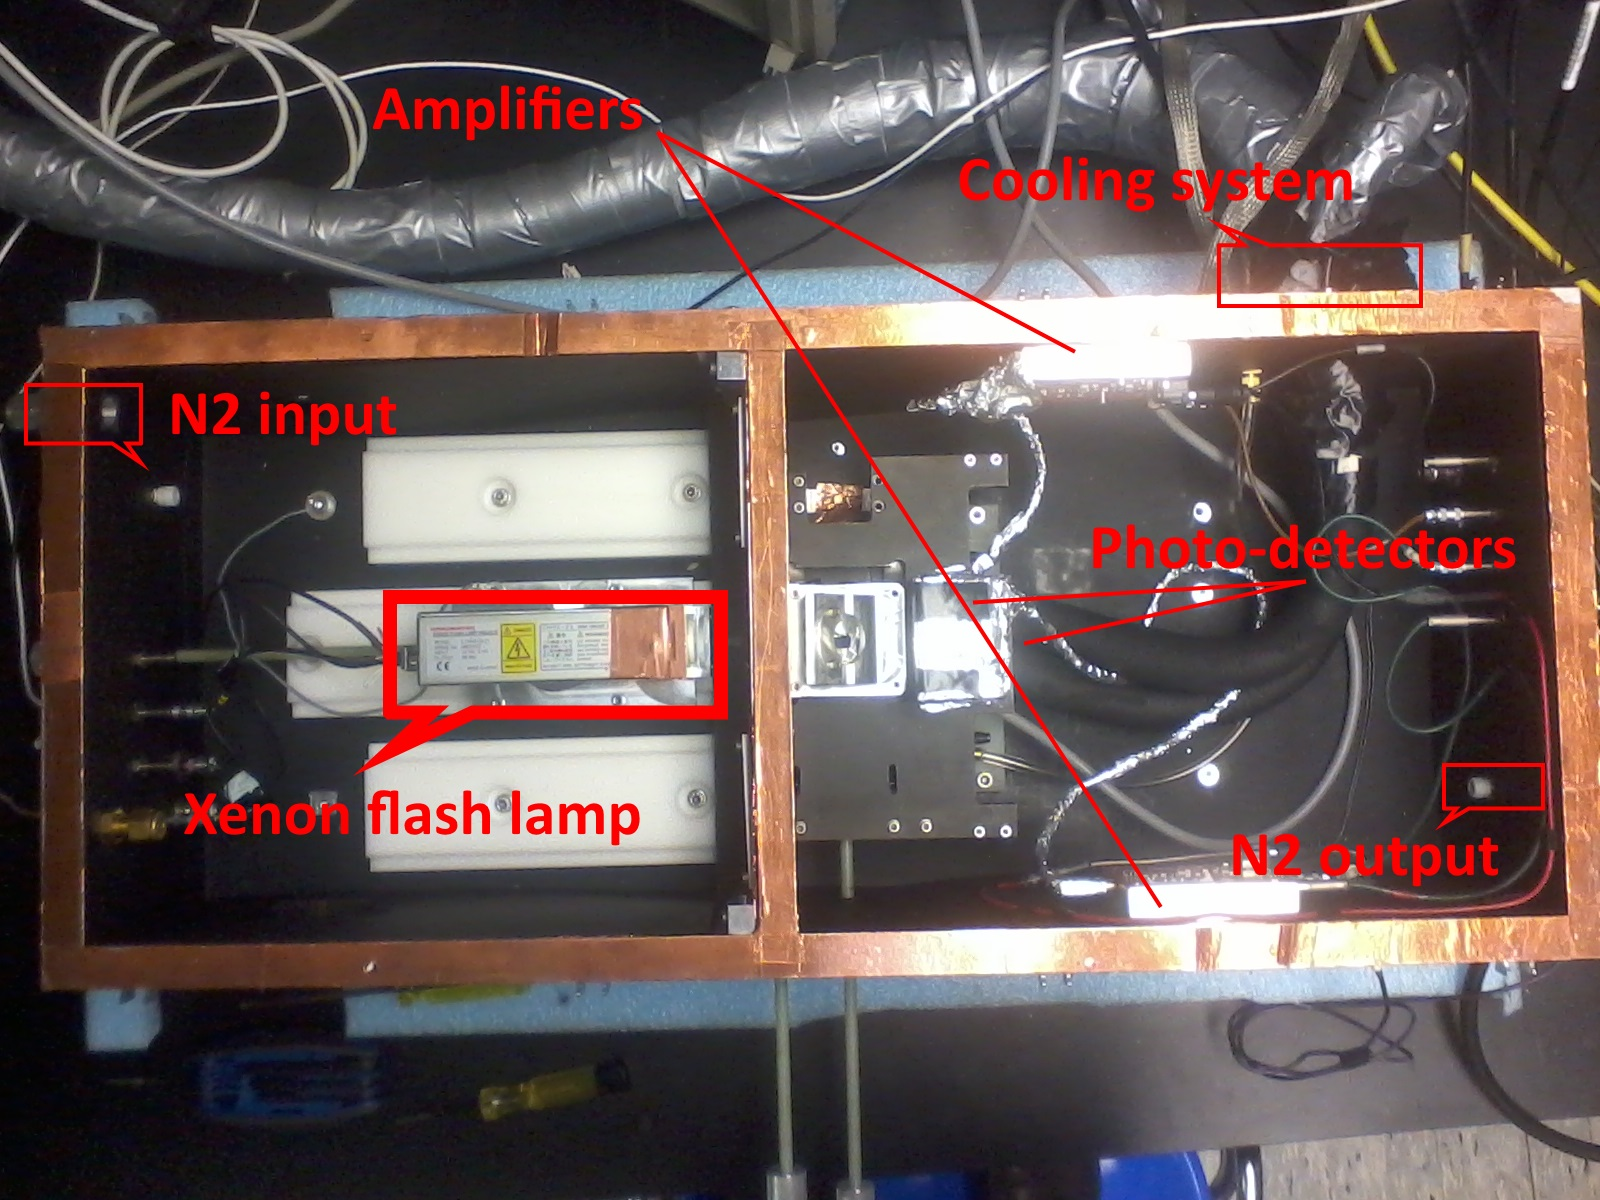
\includegraphics[totalheight=.35\textwidth,trim=0cm 7cm 0cm 2.5cm, clip=true,]{../Pictures/blabla/box.jpg}%trim=10cm 4cm 1cm 12cm, clip=true, 
  \caption{An aluminium box contains a \xfl and two photodetectors.}
  \label{fig:DN_AP_CT}
  \end{figure}
  
  The appendix A gives more details about the setup/The 
  
  \subsection{Treatment of the light}
  
  A Hamamatsu L11035-03-21 Xenon flash lamp module was utilized as a light source in a nitrogen-filled, light-tight box to simulate the 
  ultraviolet conditions of the future experiment. 
  The amount of light hitting the photodetectors was managed by a square wave pulse generator, otherwise saturation of the signal from the 
  photodetectors occurs. 
  \\
  To control light output, and thus the number of photons reaching the photodetectors, we could move out the lamp away from the surface of the detector 
  since intensity of light drops off as one over distance suqarred (make a plot). We could also set the voltage discharge on the lamp 
  by adding an external voltage supply line. 
  
  \begin{figure}[!hbtp]
  \centering
  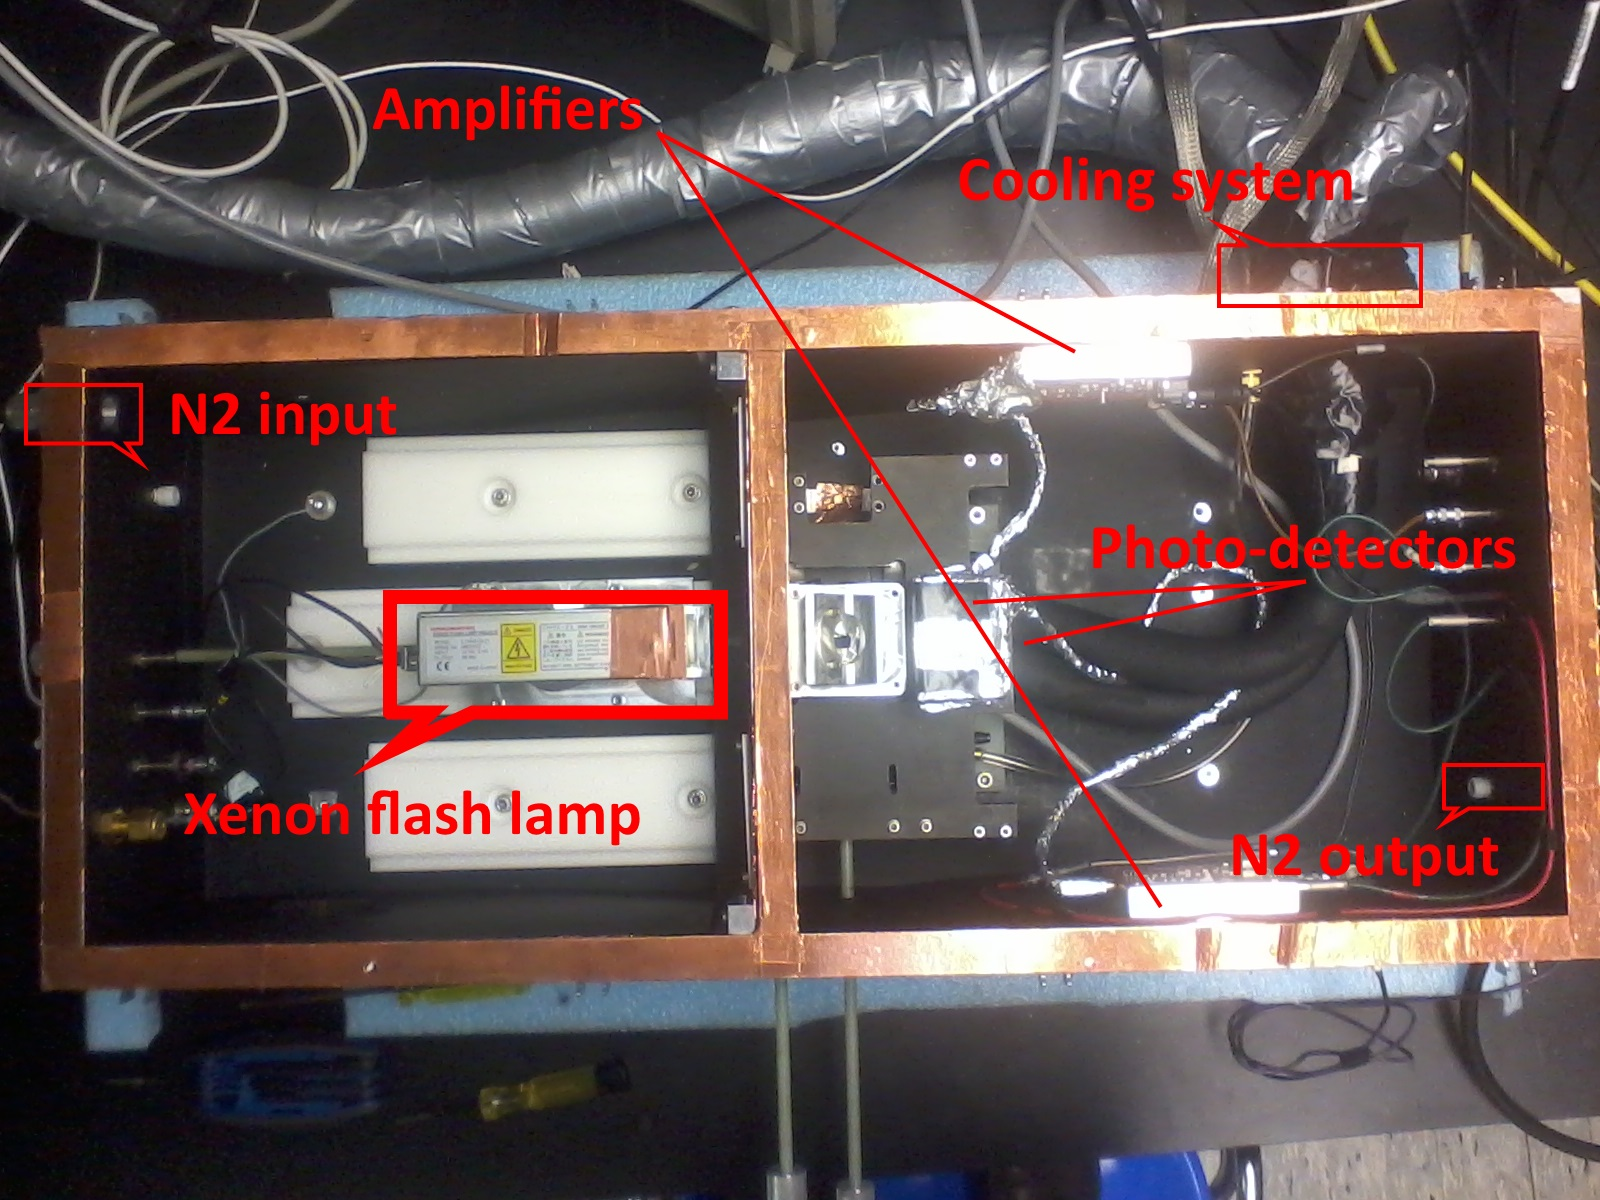
\includegraphics[totalheight=.35\textwidth,trim=0cm 7cm 0cm 2.5cm, clip=true,]{../Pictures/blabla/box.jpg}%trim=10cm 4cm 1cm 12cm, clip=true, 
  \caption{An external voltage supply line allow controling the \xfl.}
  \label{fig:external_supply_line}

  For all our measurements, the position of the lamp and the external voltage were set at 20 mm from the metal divider of the box and at 2.8 V, respectively.
  Then the light was collimated by a 5 mm hole, filtered, and then interacts with a beam splitter (BS). The beam splitter separated the 
  incoming beam into two 
  equal beams which reached the surface of each photodetector at the same time. 
  \\
  Two pictures side by side. one bs and other filter.  
  
  \begin{figure}[!hbtp]
  \centering
  \begin{subfigure}{.5\textwidth}
    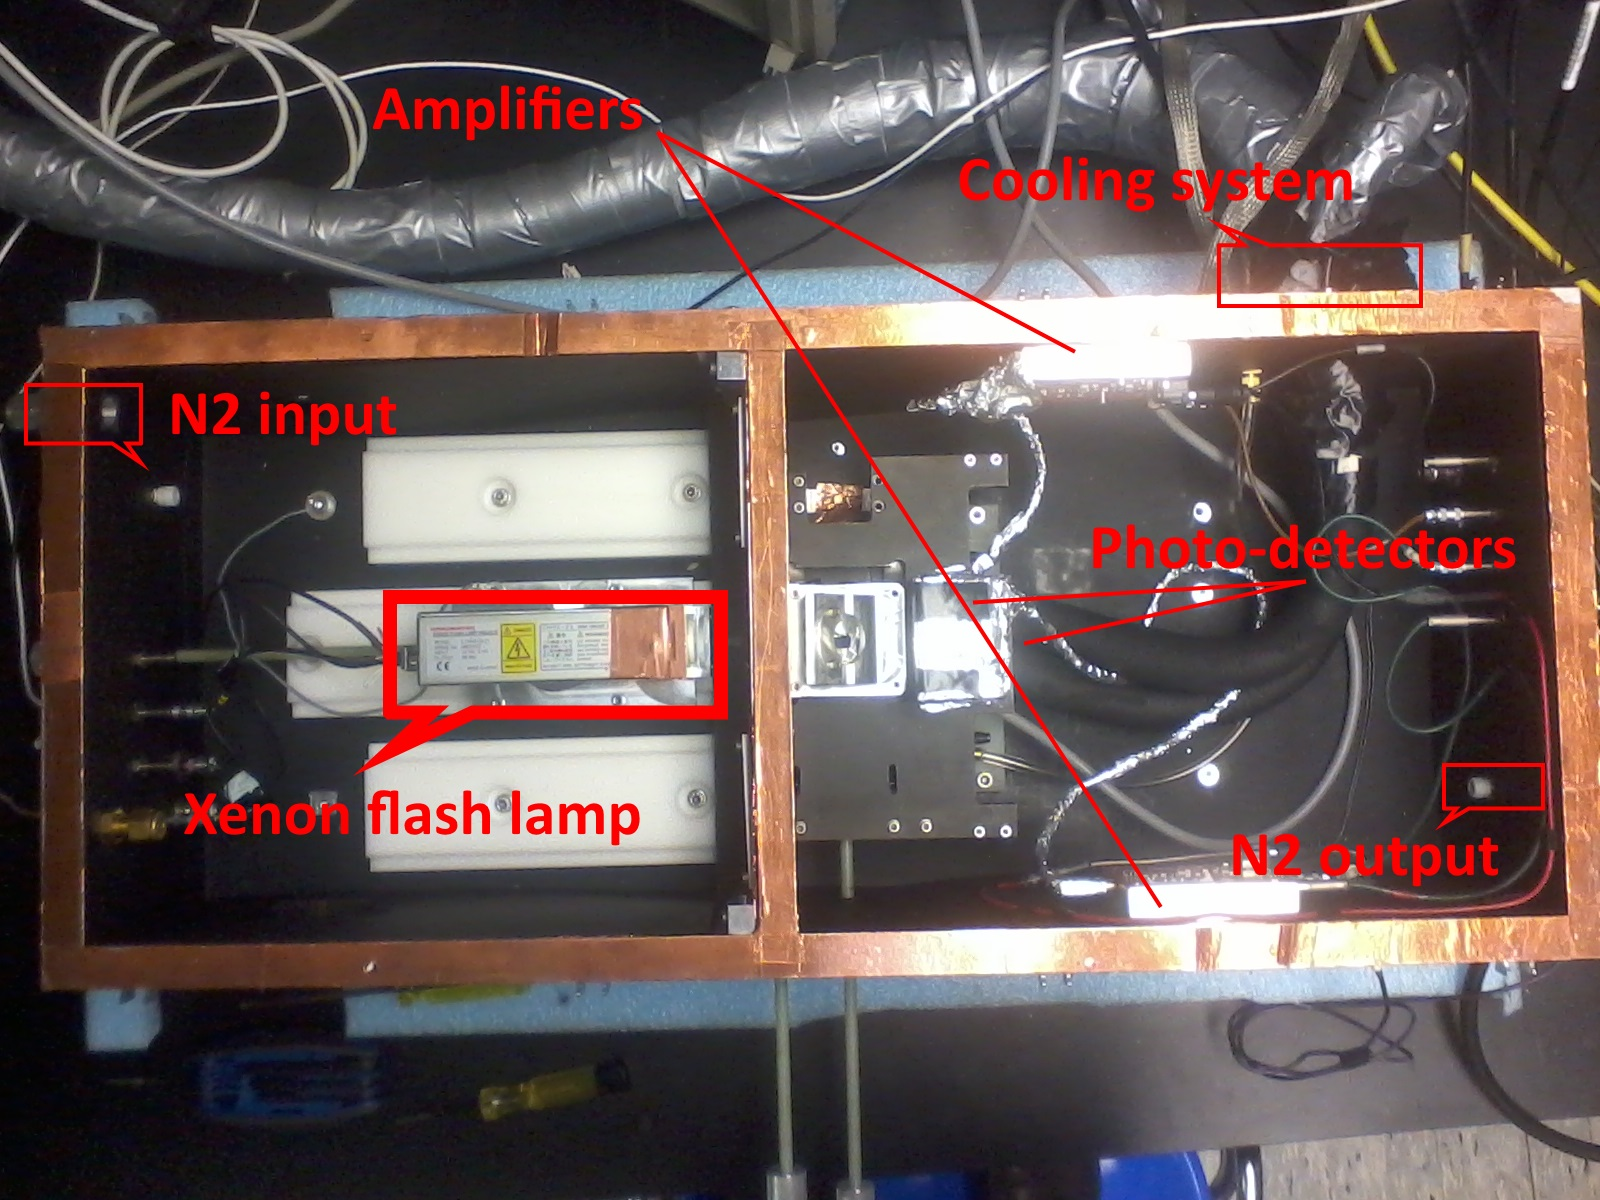
\includegraphics[totalheight=.35\textwidth,trim=0cm 7cm 0cm 2.5cm, clip=true,]{../Pictures/blabla/box.jpg}%trim=10cm 4cm 1cm 12cm, clip=true, 
    \caption{The incoming beam reachs the surface of each detectors due to the beam splitter.}
    \label{fig:beam_splitter}
  \end{subfigure}%
  \begin{subfigure}{.5\textwidth}
    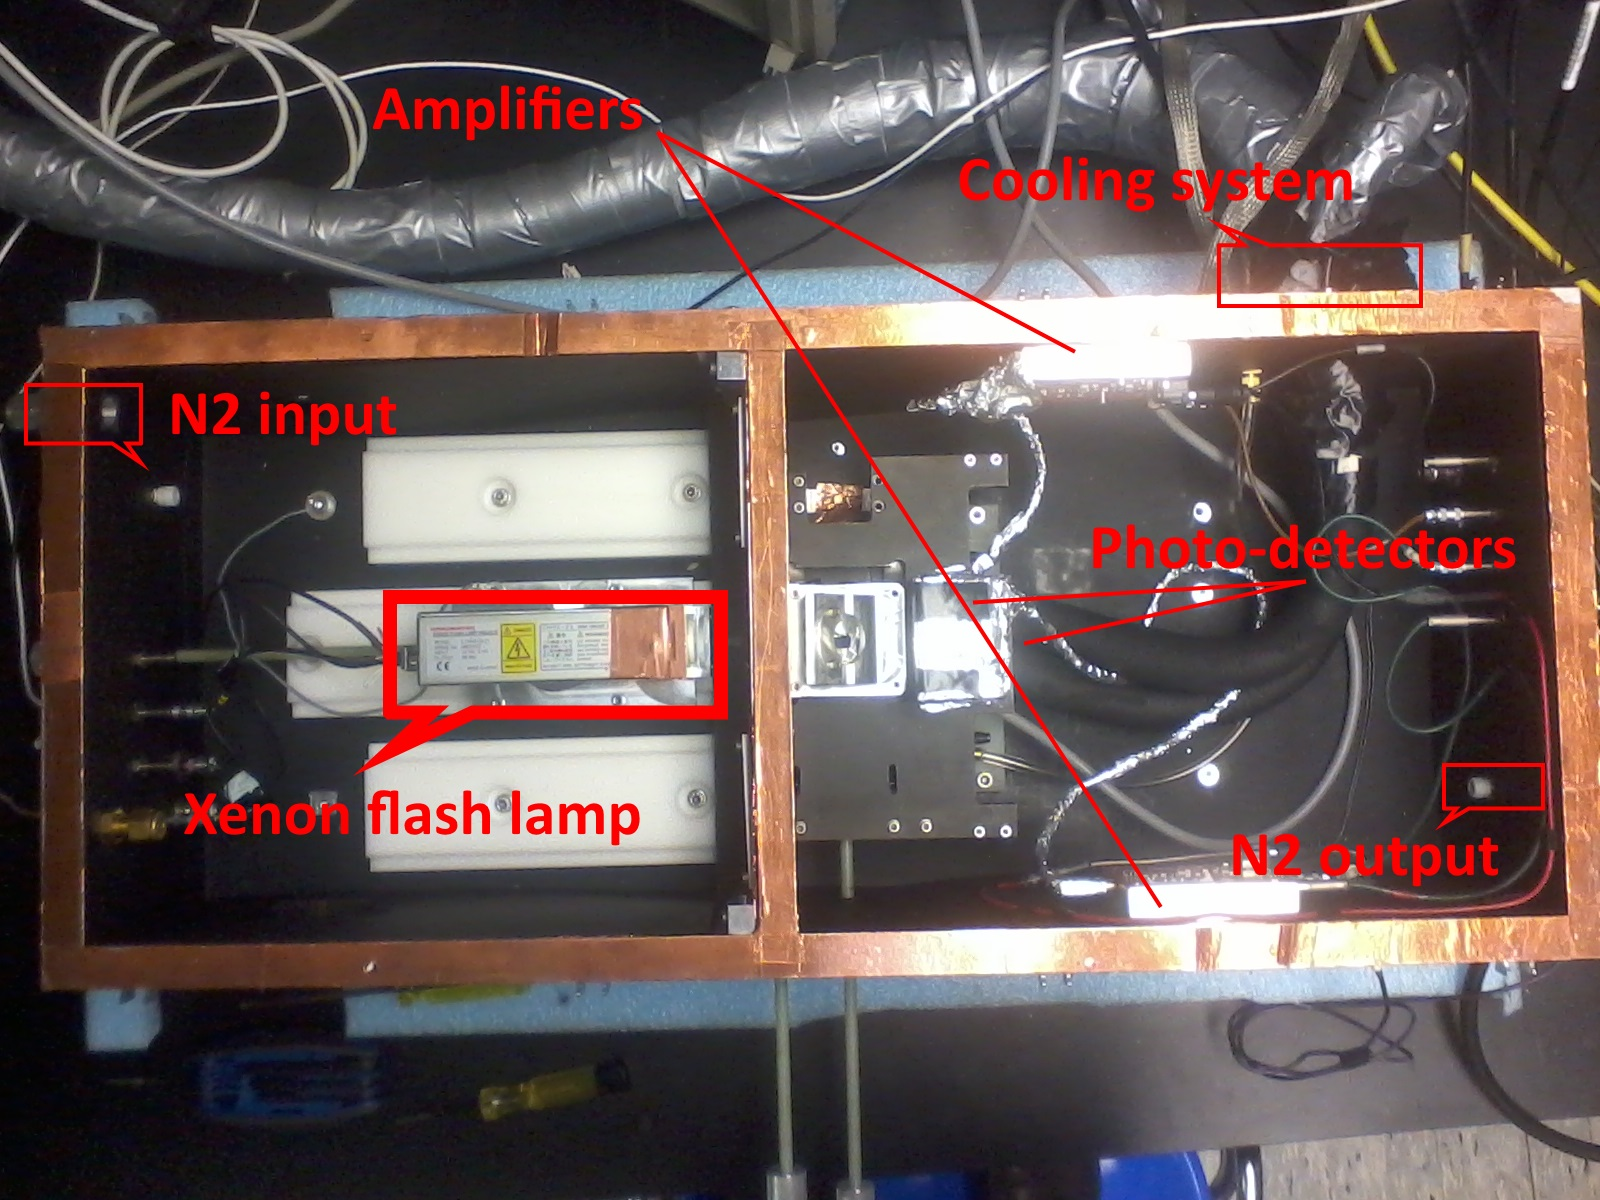
\includegraphics[totalheight=.35\textwidth,trim=0cm 7cm 0cm 2.5cm, clip=true,]{../Pictures/blabla/box.jpg}
    \caption{One of the three filters used to atenuate the light.}
    \label{fig:filters}
  \end{subfigure}
  \end{figure}
  
  
  The \xfl emits a spectrum of light in visible-light visible regions. With an external power supply, the lamp send a flash of 10 µs each 
  10 ms. The appendix gives the pulse shape of the \xfl.\\
  A filter select the 175 nm wavelength (UV region). 
  A test was made to ensure that no visible light from that lamp could reach the photo-detectors\footnote{name.} sensitive to the visible wavelength. 
  Otherwise such light could have got wronf our results for the efficiency.
  This filter also attenuated the light of the \xfl by 20\%. Then two other 
  identical filters were added to provide additional attenuations (the light reaching the photo-detectors was still too intense). 
  \\
  
  \centering
  \begin{figure}[!hbtp]  
    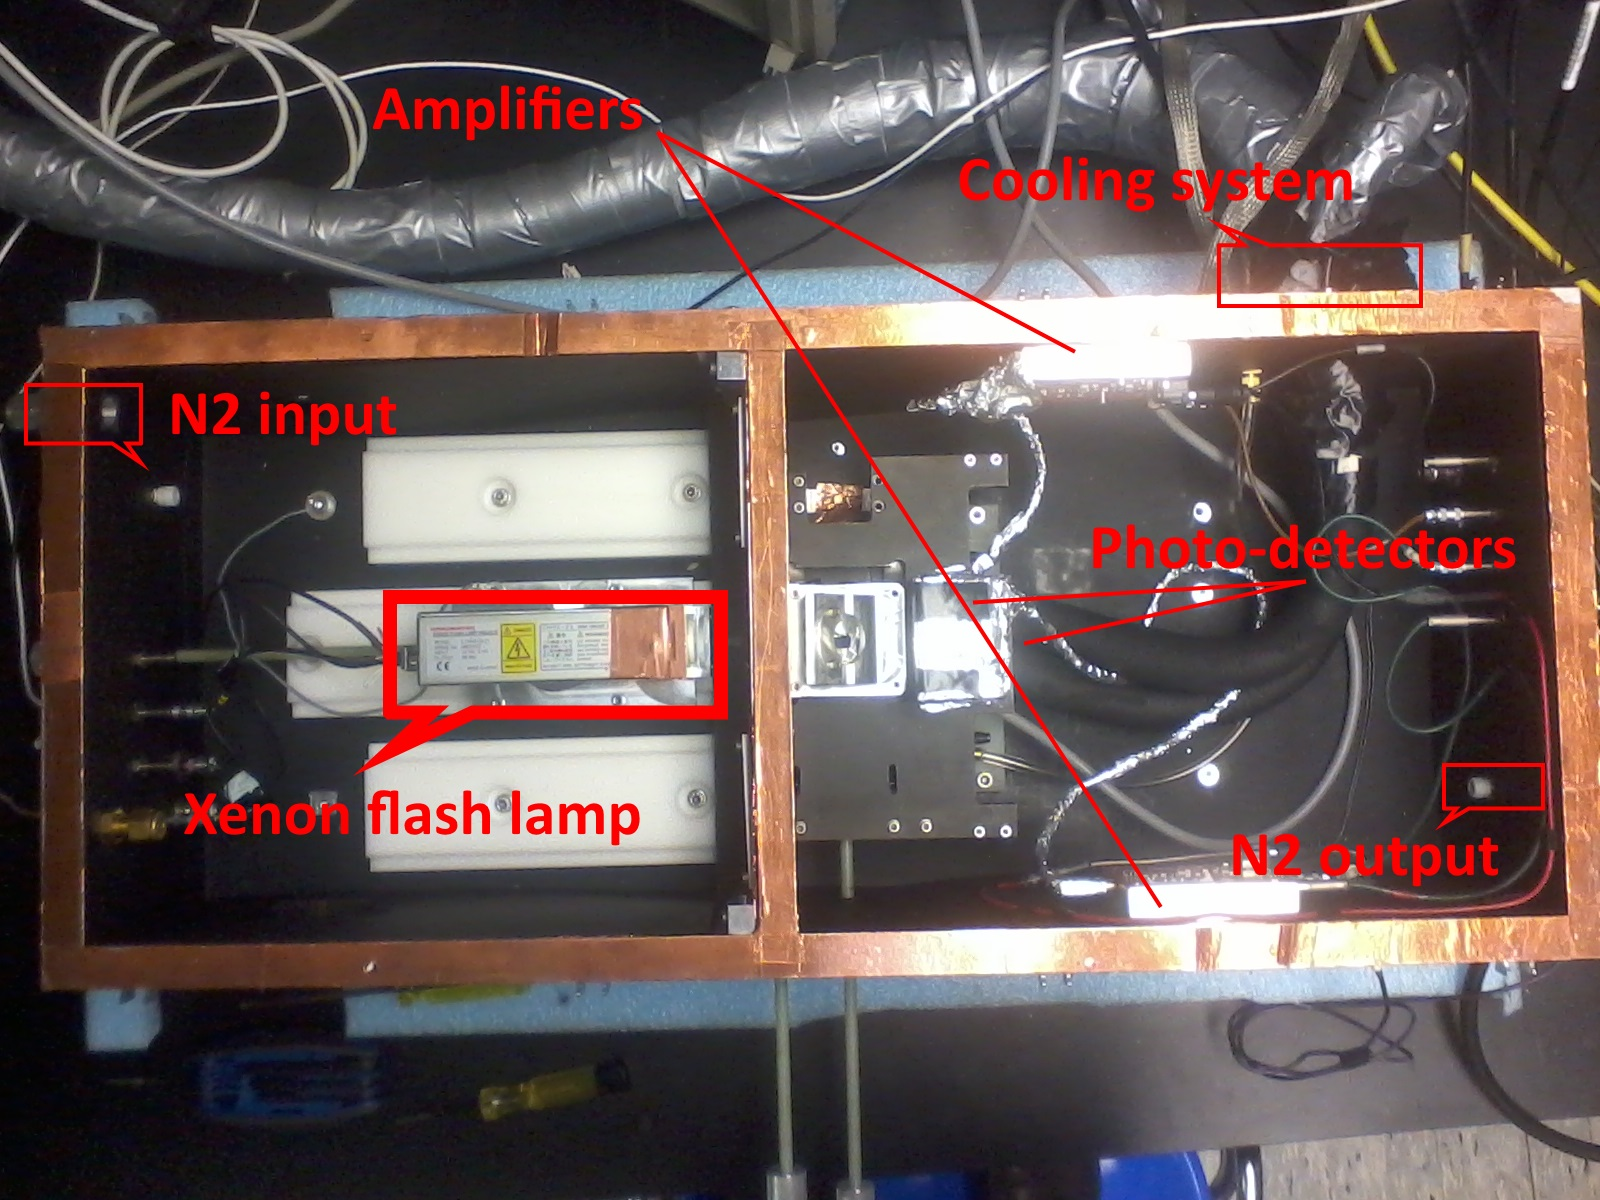
\includegraphics[totalheight=.35\textwidth,trim=0cm 7cm 0cm 2.5cm, clip=true,]{../Pictures/blabla/box.jpg}
    \caption{The closest filter near the lamp select the VUV region.}
    \label{fig:filter_specification}
  \end{figure}
  
  As photons of this wavelength have an attenuation length of only a few mm, the box was filled with N2 gas. The second advanatge of using 
  N2 is to avoid frost on the surface of the cooling photo-detectors on the bottom.
   
  \centering
  \begin{figure}[!hbtp]  
    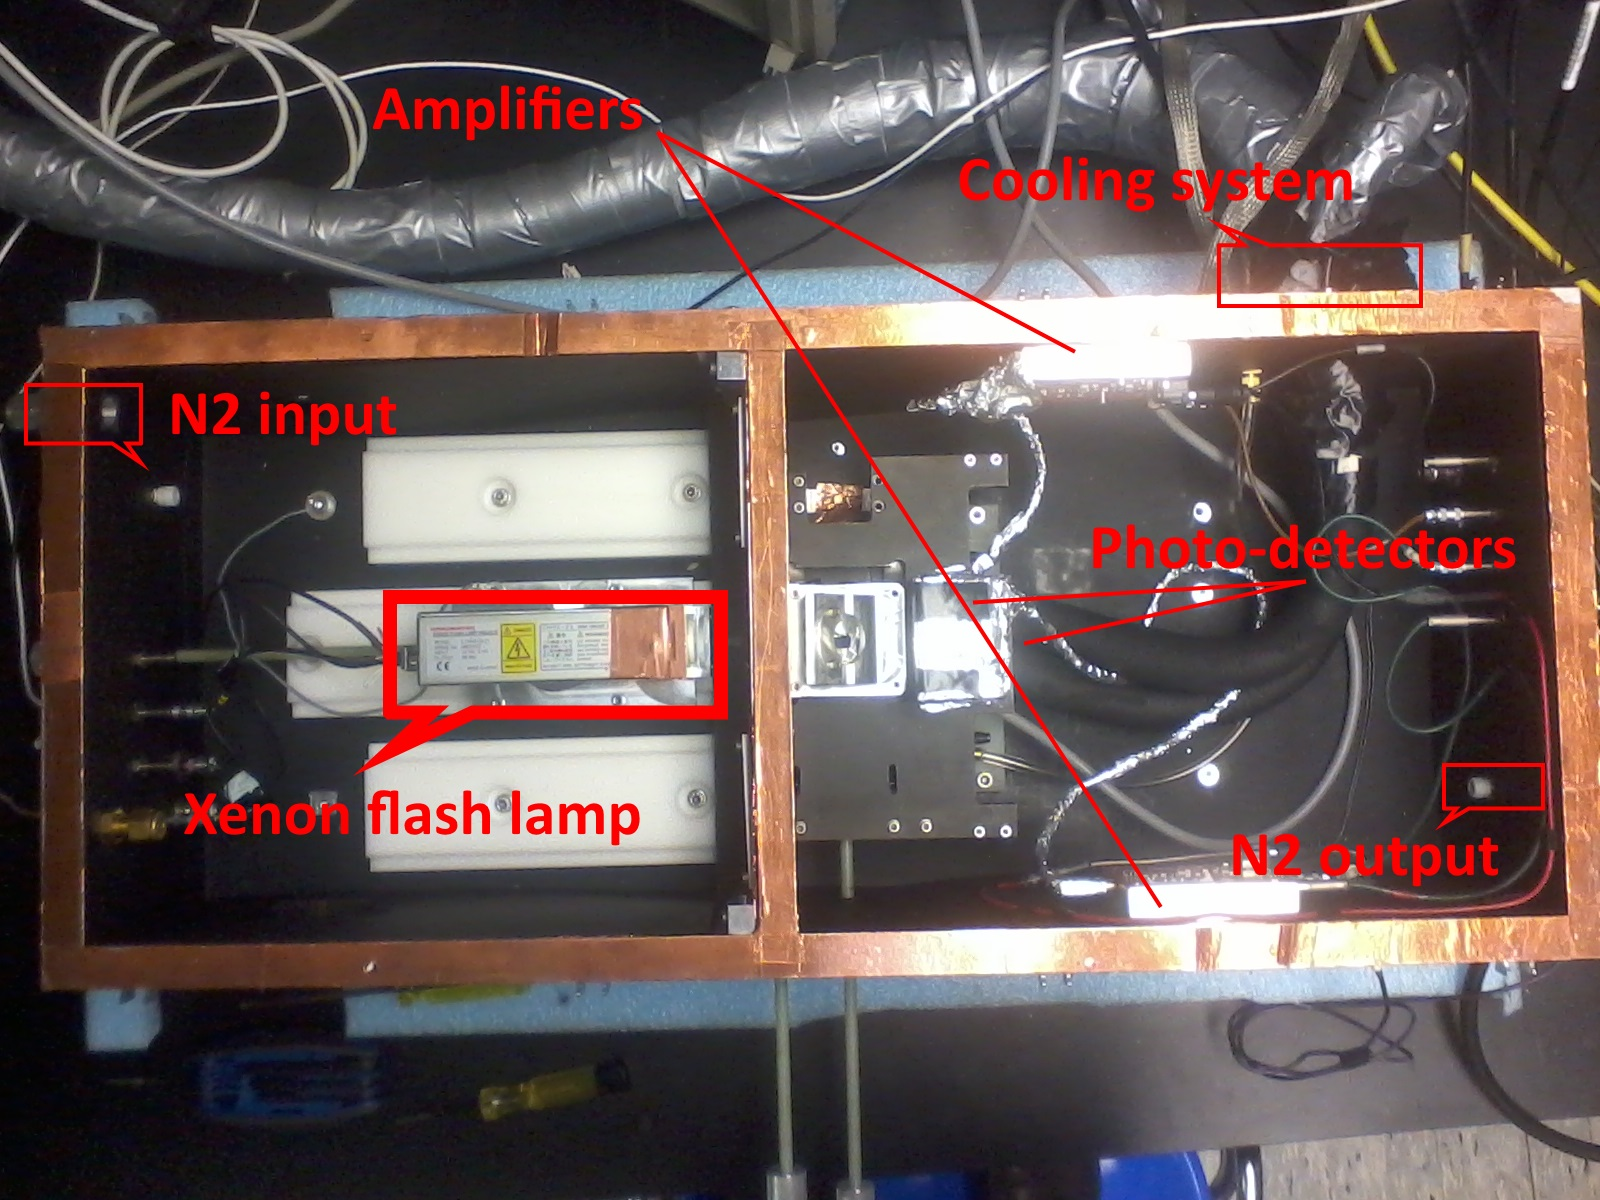
\includegraphics[totalheight=.35\textwidth,trim=0cm 7cm 0cm 2.5cm, clip=true,]{../Pictures/blabla/box.jpg}
    \caption{N2 from that bottle fills the box.}
    \label{fig:filter_specification}
  \end{figure}
  
  
  \subsection{Photo-detectors and cooling system}
  
  Two photo-detectors were used for each run to calculate the efficiency.\\
  The one on the top allow ensuring that the light remind constant over the time. For that we used a VUV2 SIPM from Hammatsu.
  
  \centering
  \begin{figure}[!hbtp]  
    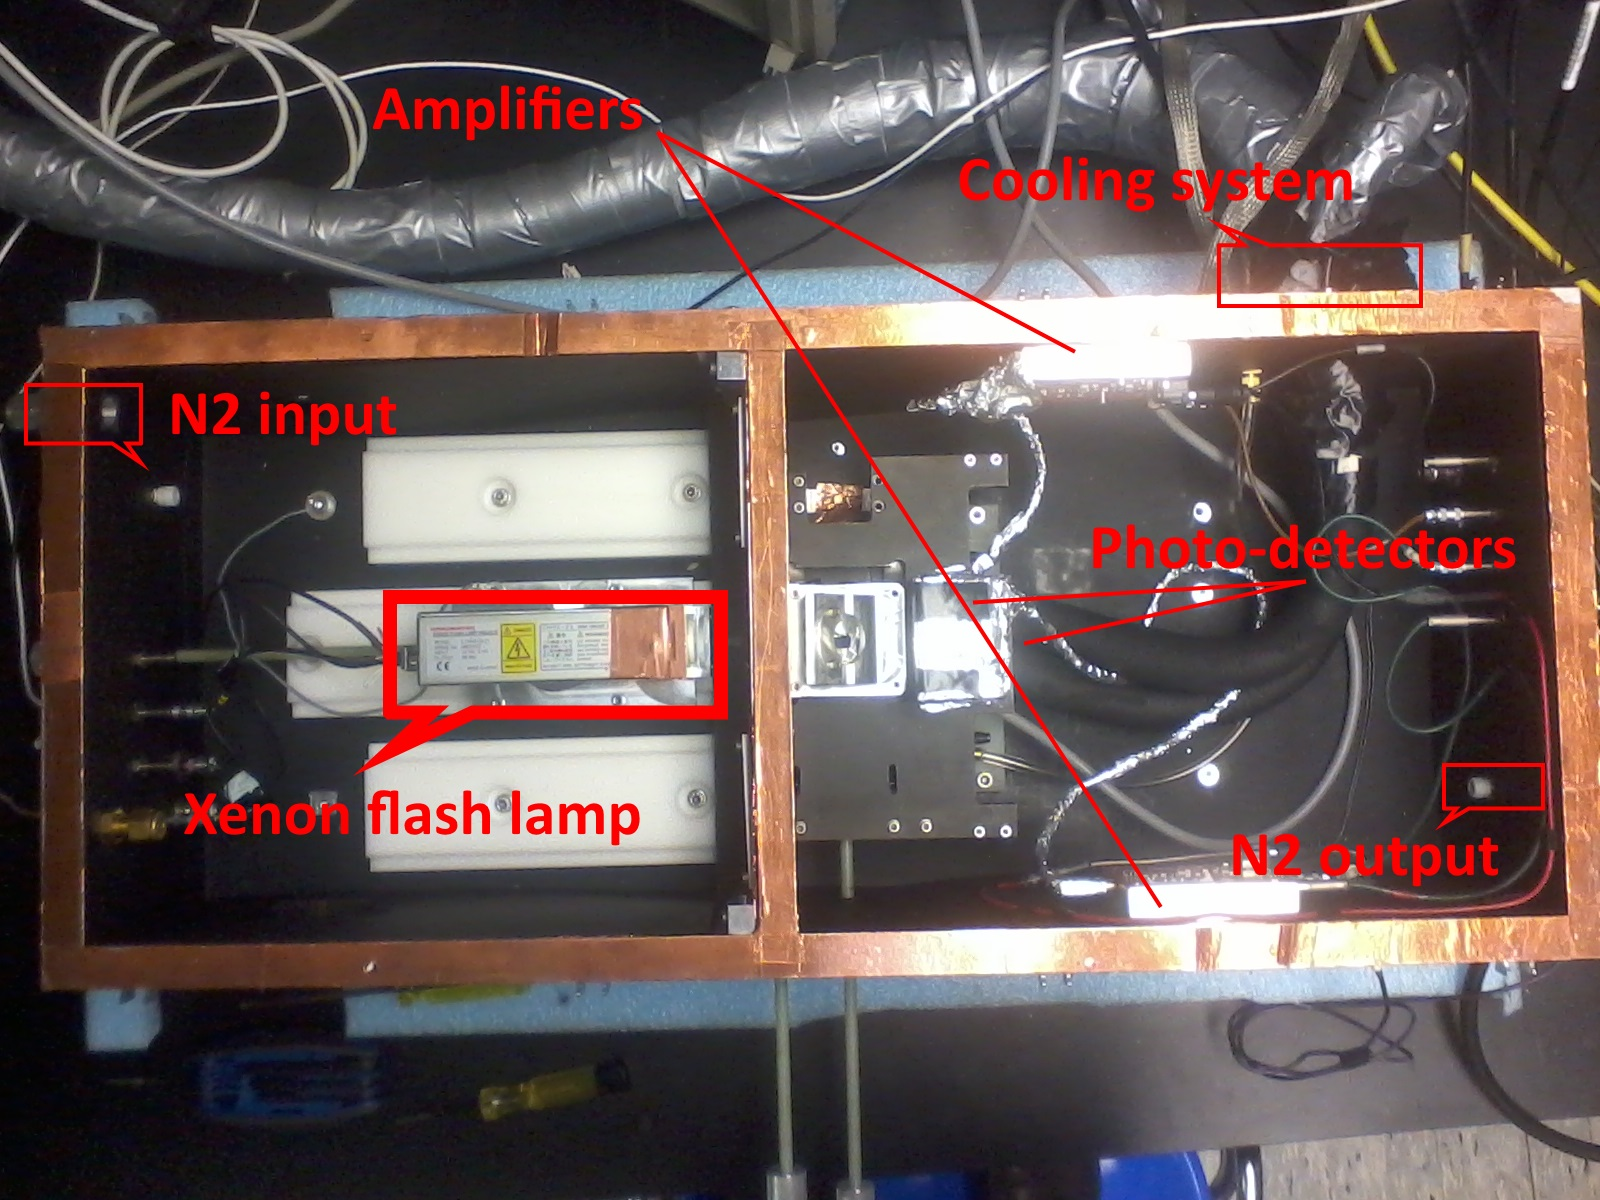
\includegraphics[totalheight=.35\textwidth,trim=0cm 7cm 0cm 2.5cm, clip=true,]{../Pictures/blabla/box.jpg}
    \caption{A VUV2 SiPM on the top let check if the  light from the lamp is constant.}
    \label{fig:top}
  \end{figure}
  
  We choose that one beacaue the dark noise rate\footnote{see section.} is quiet low at room temperature (20C). So it is possible 
  to calculate the relative efficiency of that detector at such temperature./So the efficiency of that photo-detector is not perturbé
  due to a high rate of dark noise\footnote{see section.}
  
  The photo-detector on the bottom were characterize (calculation of the efficiency at -100C, of the dark noise and the number of 
  correlated pulse rate).\\
  A cooling system allow working at such low temperature and the photo-detector to characterize was laying on a chock. A plastic board 
  with bad termo conductivity holds the whole cooling shock to avoid thermal flee.\\
    
  \begin{figure}[!hbtp]
  \centering
  \begin{subfigure}{.5\textwidth}
    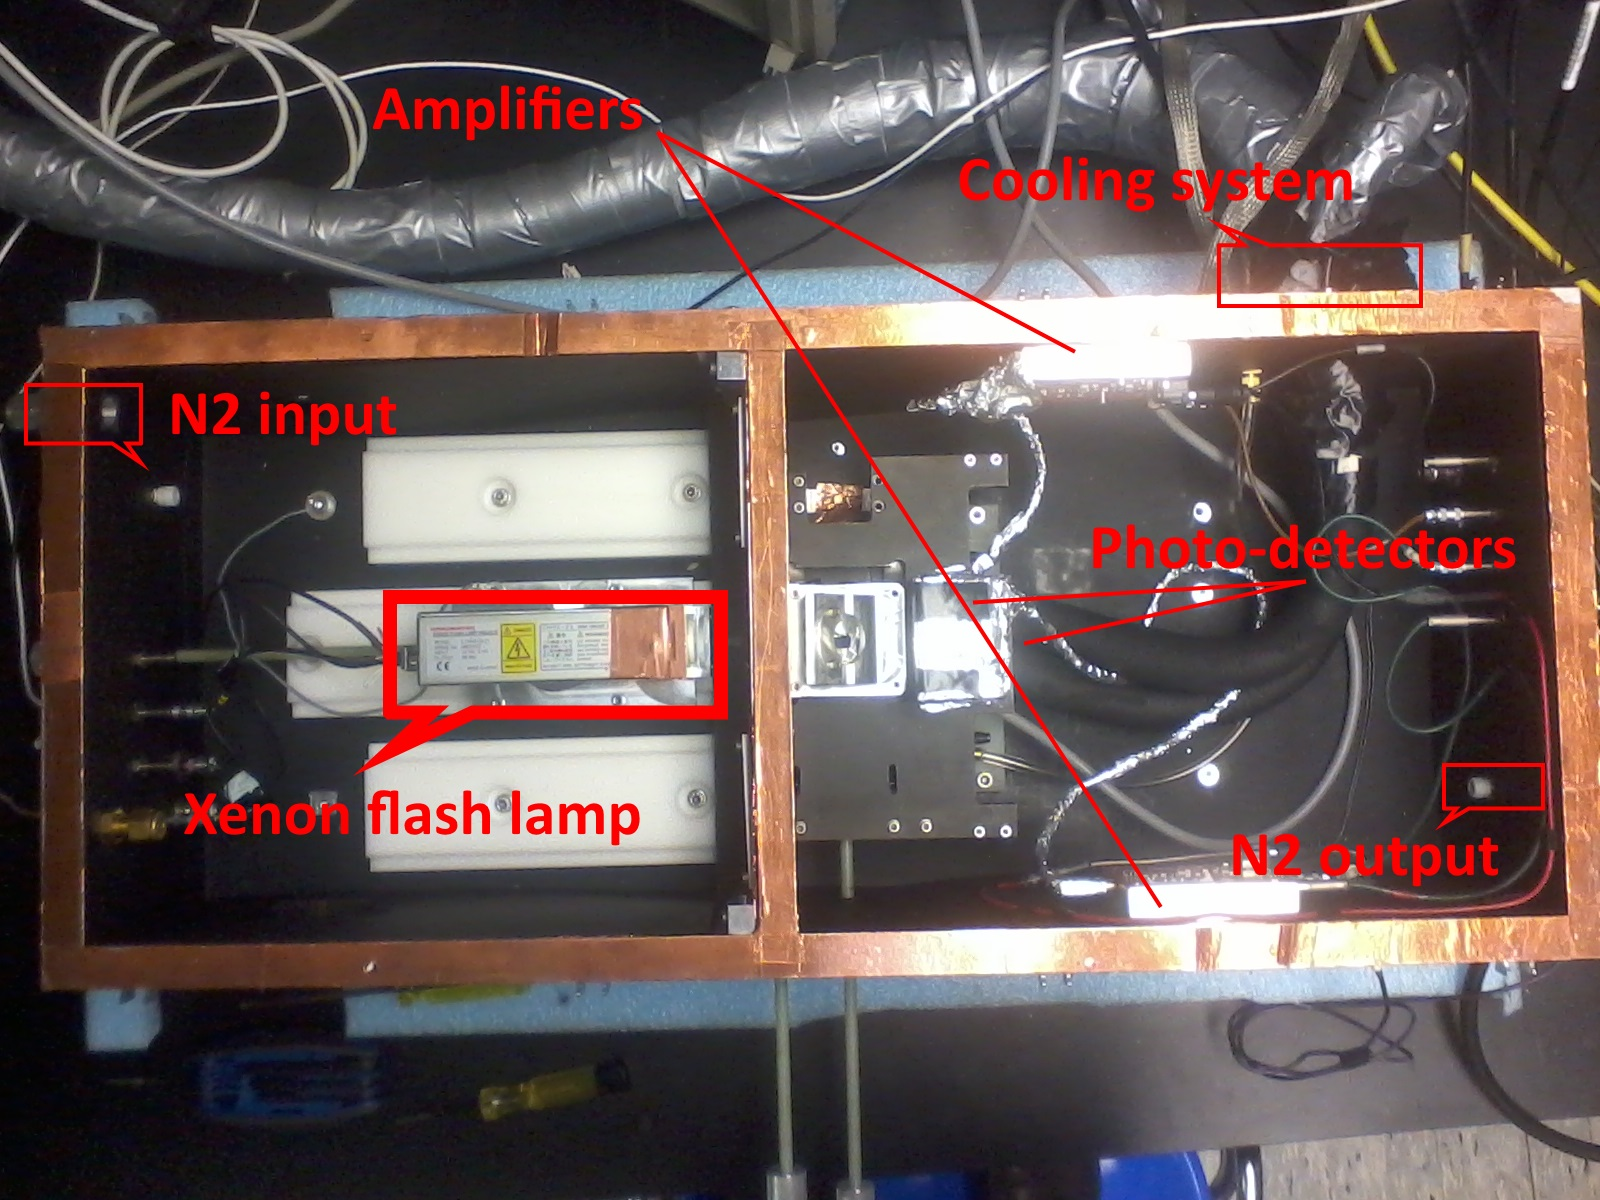
\includegraphics[totalheight=.35\textwidth,trim=0cm 7cm 0cm 2.5cm, clip=true,]{../Pictures/blabla/box.jpg}%trim=10cm 4cm 1cm 12cm, clip=true, 
    \caption{The cooling system let work up to -110C.}
    \label{fig:beam_splitter}
  \end{subfigure}%
  \begin{subfigure}{.5\textwidth}
    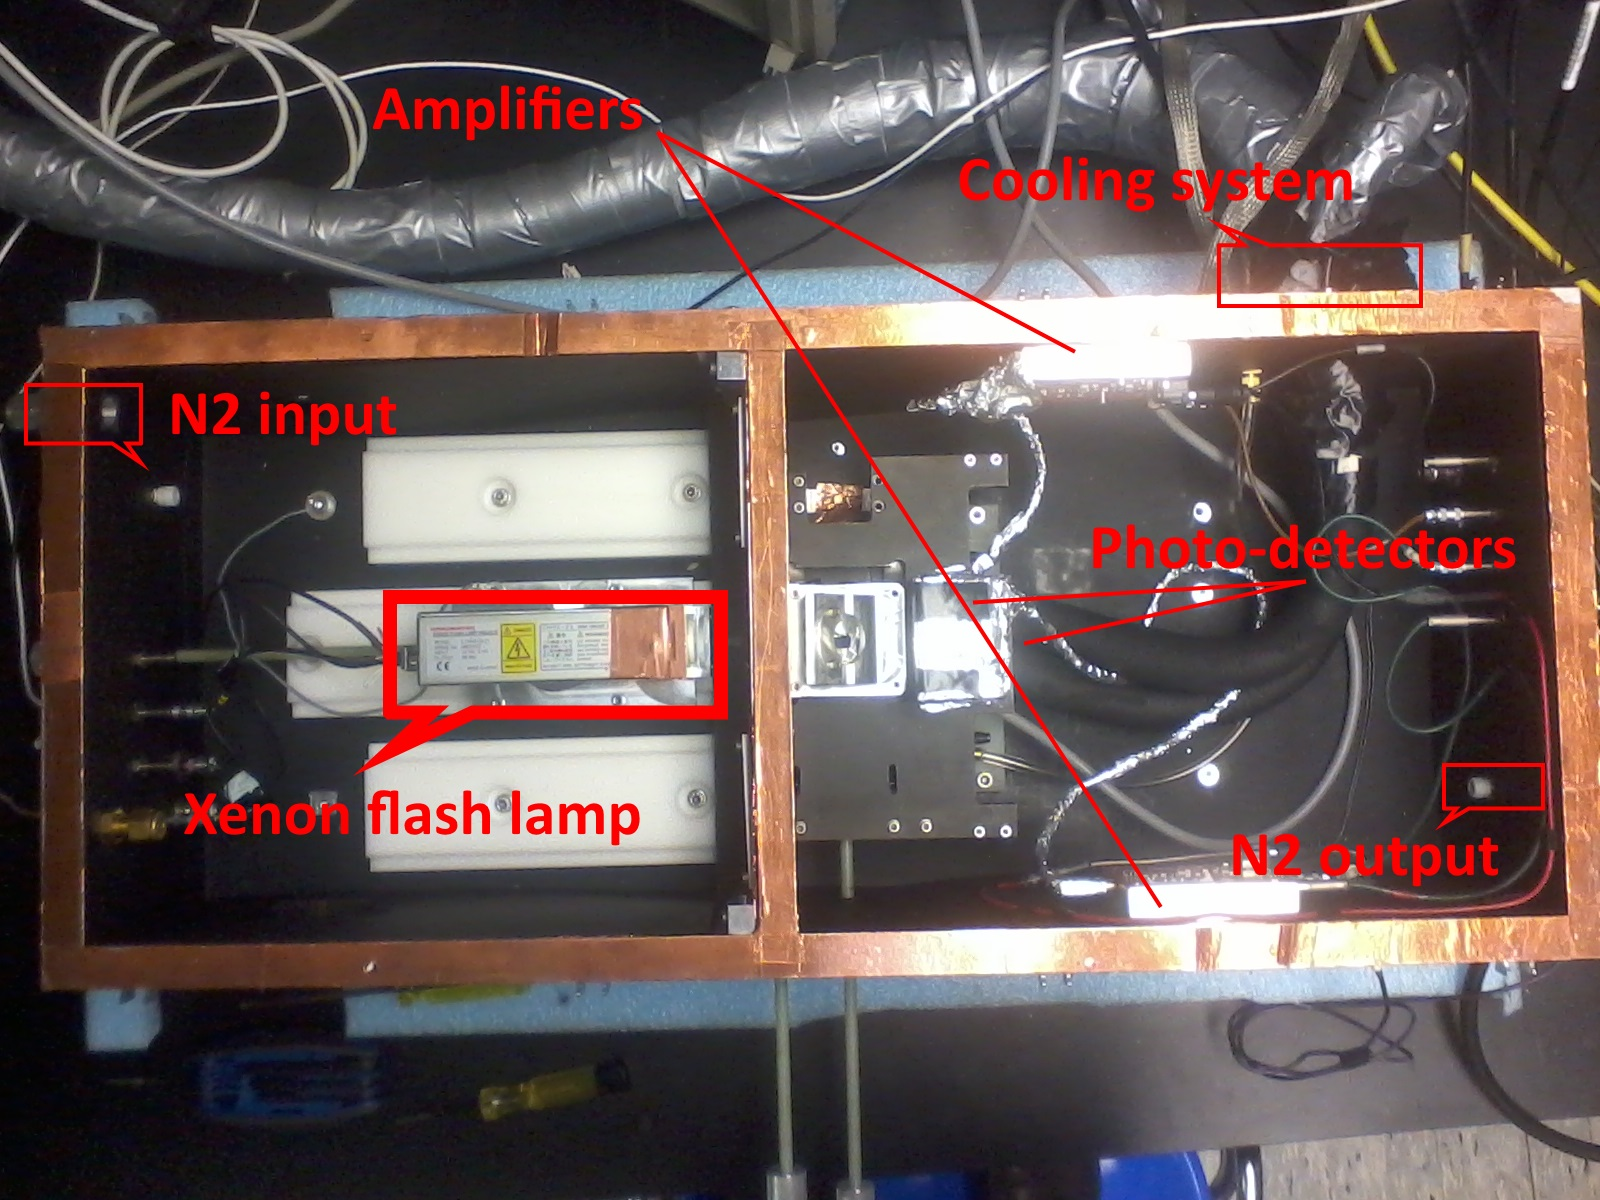
\includegraphics[totalheight=.35\textwidth,trim=0cm 7cm 0cm 2.5cm, clip=true,]{../Pictures/blabla/box.jpg}
    \caption{ VUV3 SIPM of HAMMAMATSU.}
    \label{fig:cooing system}
  \end{subfigure}
  \end{figure}  
  
  Several different SiPM were tested to select the best one/ the more suitable one for nEXO.
  
  \begin{figure}[!hbtp]
  \centering
  \begin{tabular}{|l|c|c|c|}
  \hline
  D\'etecteur SiPM (diff\'erents fournisseurs) &Efficacit\'e &Dark Noise &Cross Talk + After Pulse\\
  \hline
  MPPC VUV2/MEG &oui &oui &oui\\
  \hline
  MPPC VUV3/MEG &non &non &non\\
  \hline
  MPPC cooted &non &- &-\\
  \hline
  KETEK 1 &- &non &non\\
  \hline
  KETEK 2 & &non &non\\
  \hline
  FDK VUV &non &non &non\\
  \hline
  FBK &- &non &non\\
  \hline
  \end{tabular}
  \end{figure}
  
  \subsection{Temperature sensors and automatisation}
  
  We noticed that the whole bow were cooling down over time when we were working at -100C, even the plastic holder.\\
  To check if that physical phenomena could have an impact on our reseults for the efficiency 10 tempererature sensors were installed inside 
  the box after calibrating them\footnote{See appendix for more details.}\\
  At was possible to record all the temperatures by using such device. 
  
  \begin{figure}[!hbtp]
  \centering
  \begin{subfigure}{.5\textwidth}
    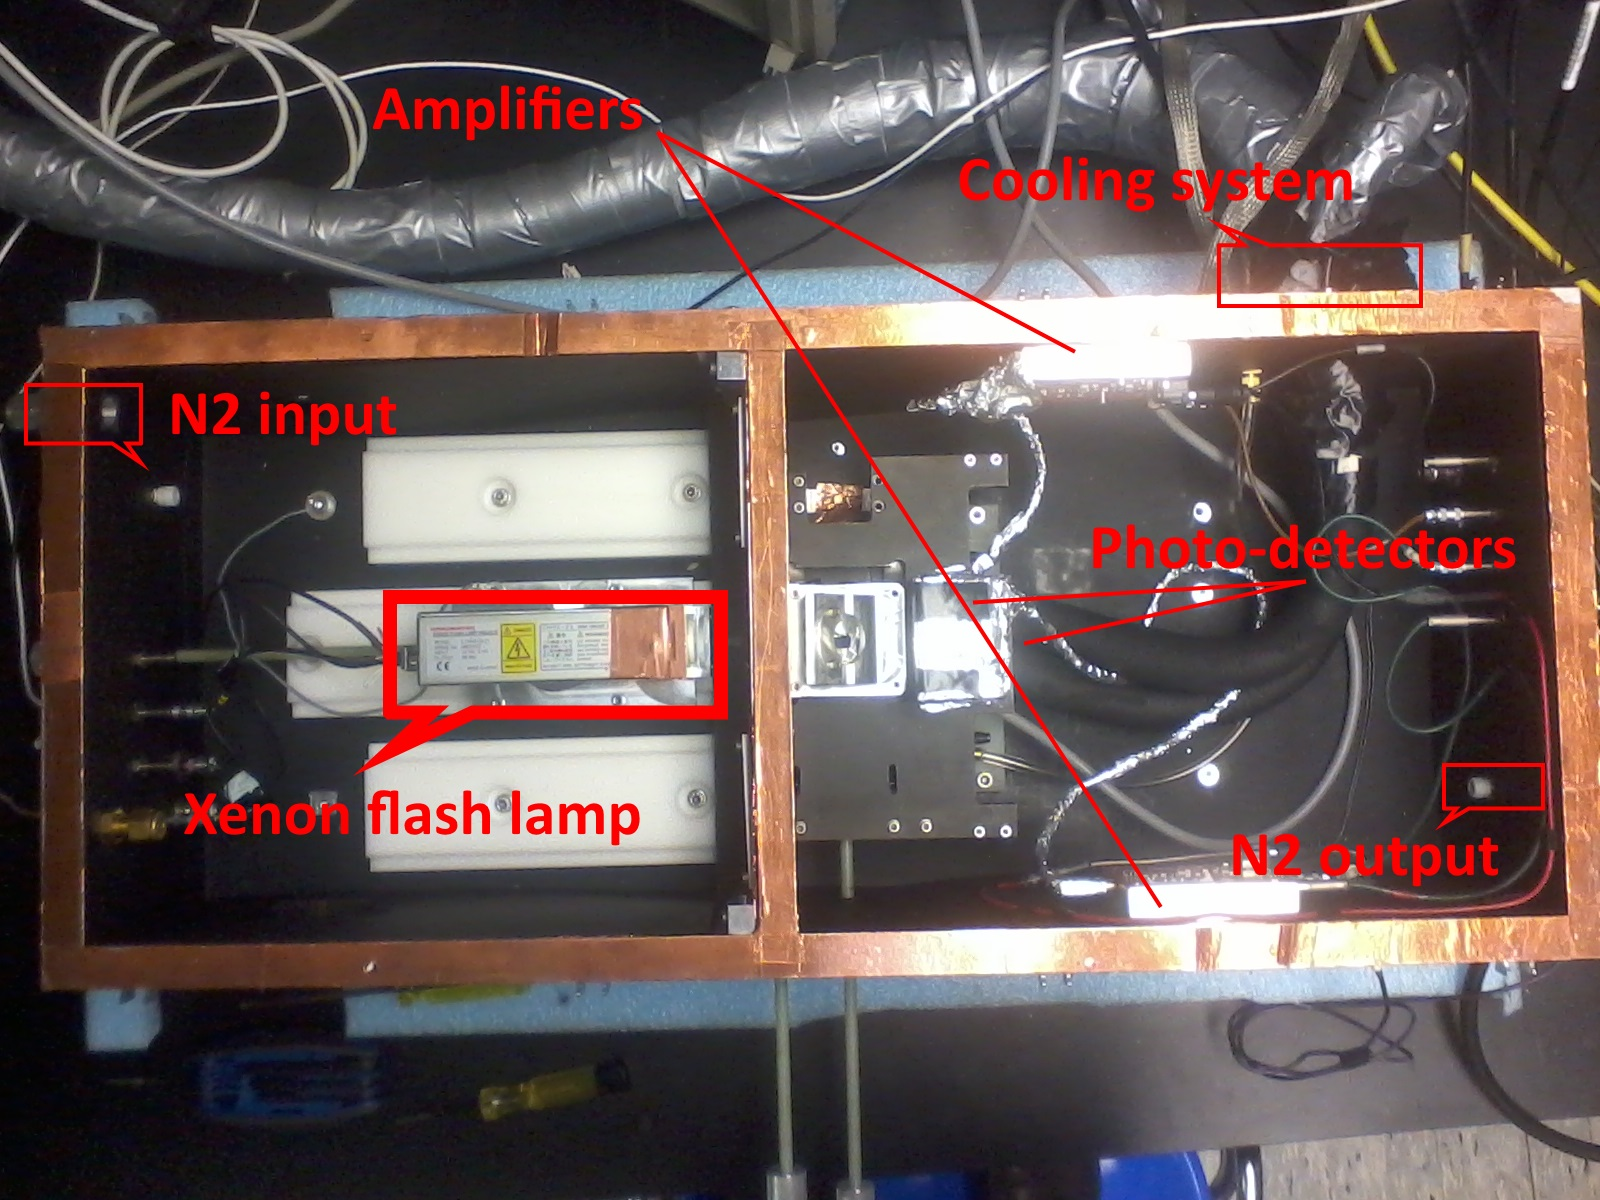
\includegraphics[totalheight=.35\textwidth,trim=0cm 7cm 0cm 2.5cm, clip=true,]{../Pictures/blabla/box.jpg}%trim=10cm 4cm 1cm 12cm, clip=true, 
    \caption{On of the ten tempearture sensors.}
    \label{fig:beam_splitter}
  \end{subfigure}%
  \begin{subfigure}{.5\textwidth}
    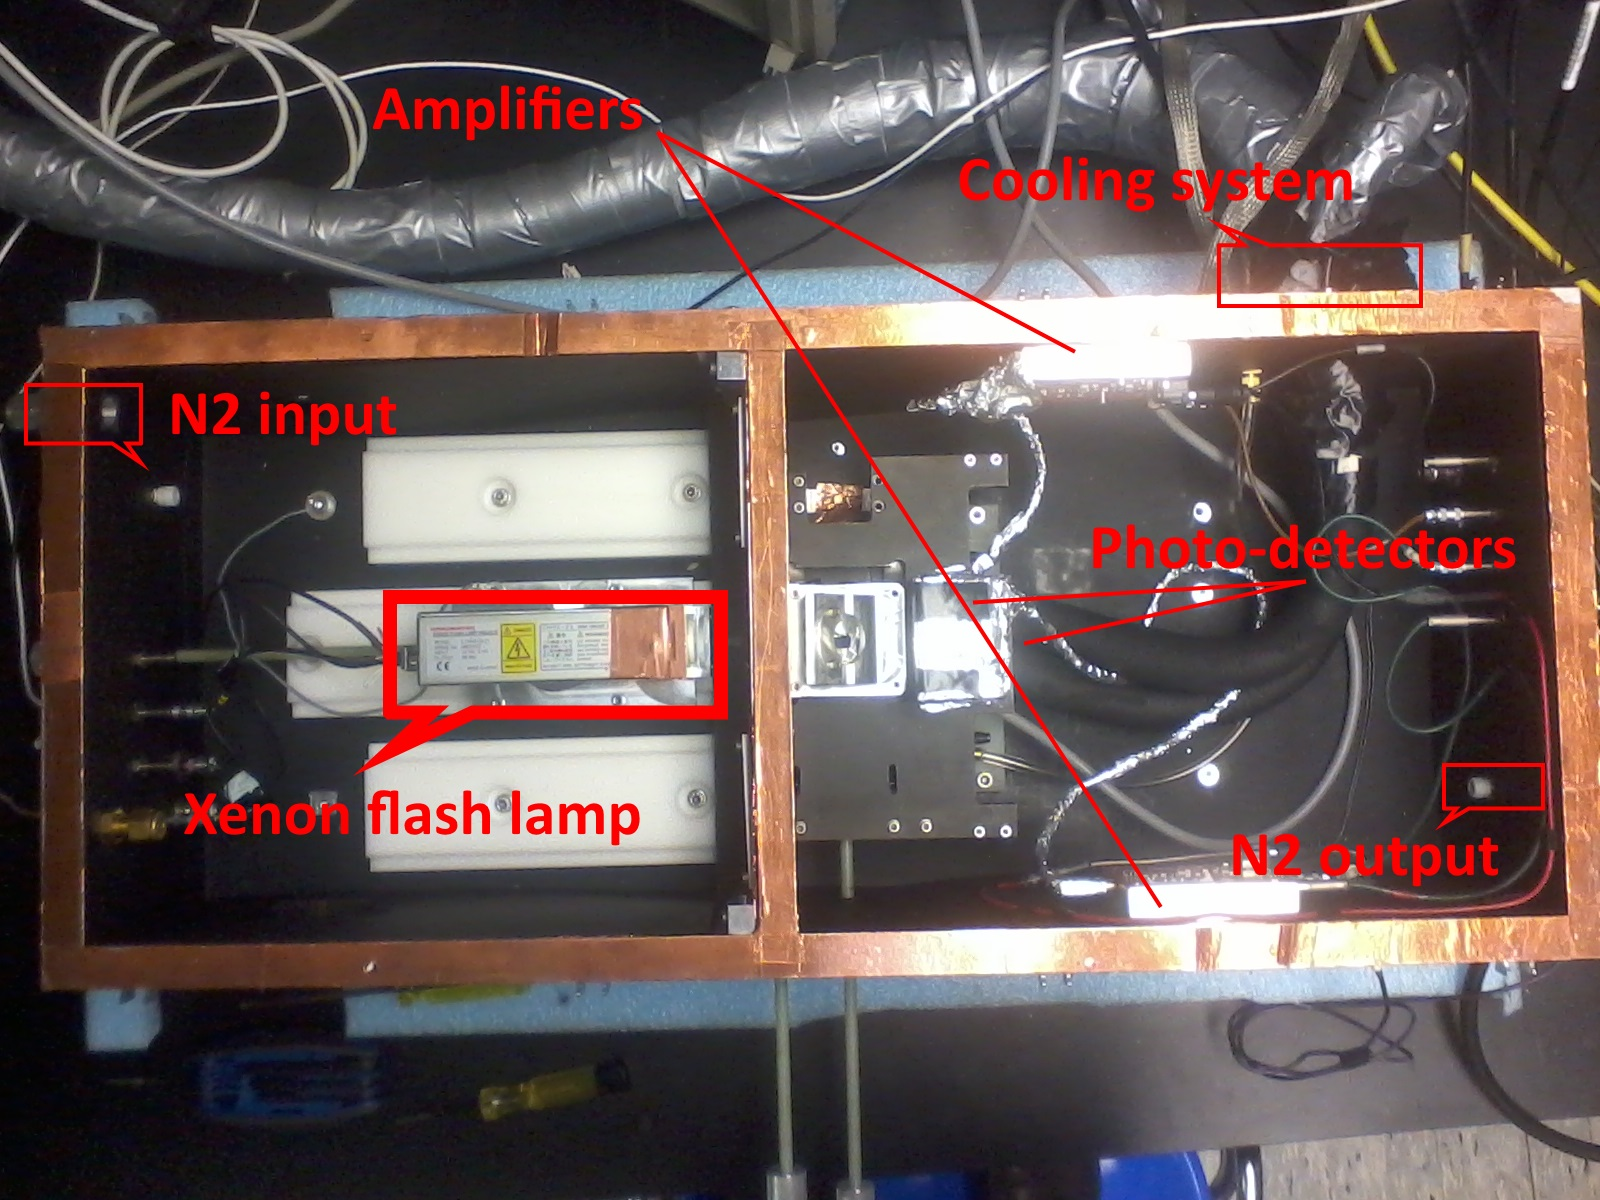
\includegraphics[totalheight=.35\textwidth,trim=0cm 7cm 0cm 2.5cm, clip=true,]{../Pictures/blabla/box.jpg}
    \caption{That device let record the different temperature.}
    \label{fig:filters}
  \end{subfigure}
  \end{figure}
  
  Also a program were written to set the volatge sended to the photo-detectors, to record the current from them and to record the 
  temperature at differentparts of the box. 
  
  \section{Silicon Photo-Multiplier}
  
  A Silicon photomultiplier (SiPM) is a photon detector (detect light). Many groups concerning sudy their applicability in many different 
  fields such as high-energy, physics calorimetry, astrophysics or medical imaging \ref{}.\\
  Compared to EXO experiment which uses conventional vacuum tube PM (PhotoMultiplier), SiPMs for nEXO experiment are a very promising 
  alternative because of the very good properties of such devices:
  
  \begin{itemize}
   \item SiPMs are insentive to magnetic fields,
   \item SiPMs' operation voltage is far lower than PMs,
   \item SiPMs' gain is \(10^6 - 10^7\) higher than PMs' gain\footnote{The resolution of energy and so the gain of the SiPM is a 
   reason why nEXO choose them},
   \item SiPMs have a very good time (ns) and photon-counting resolutions (µm) due to the size of the one pixel.
  \end{itemize}

  %SiPM properties like high gain \(10^6 - 10^7\) and sensitivity, and very good time (ns) and photon-counting (nm) resolutions
  %\.
  
  \subsection{Structure}
  
  This device consists a matrix of typically 1000 independent and equal mirco-cells (pixels) per mm\texttwosuperior{}. A pixel consists the basic 
  element of SiPMs.\\
  Each pixel are connected in parallel. They are formed out of an Avalanche PhotoDiode (APD) and a quenching resistor which is 
  connected in series to an APD. 
  
  \begin{figure}[!hbtp]
  \centering
  \begin{subfigure}{.5\textwidth}
    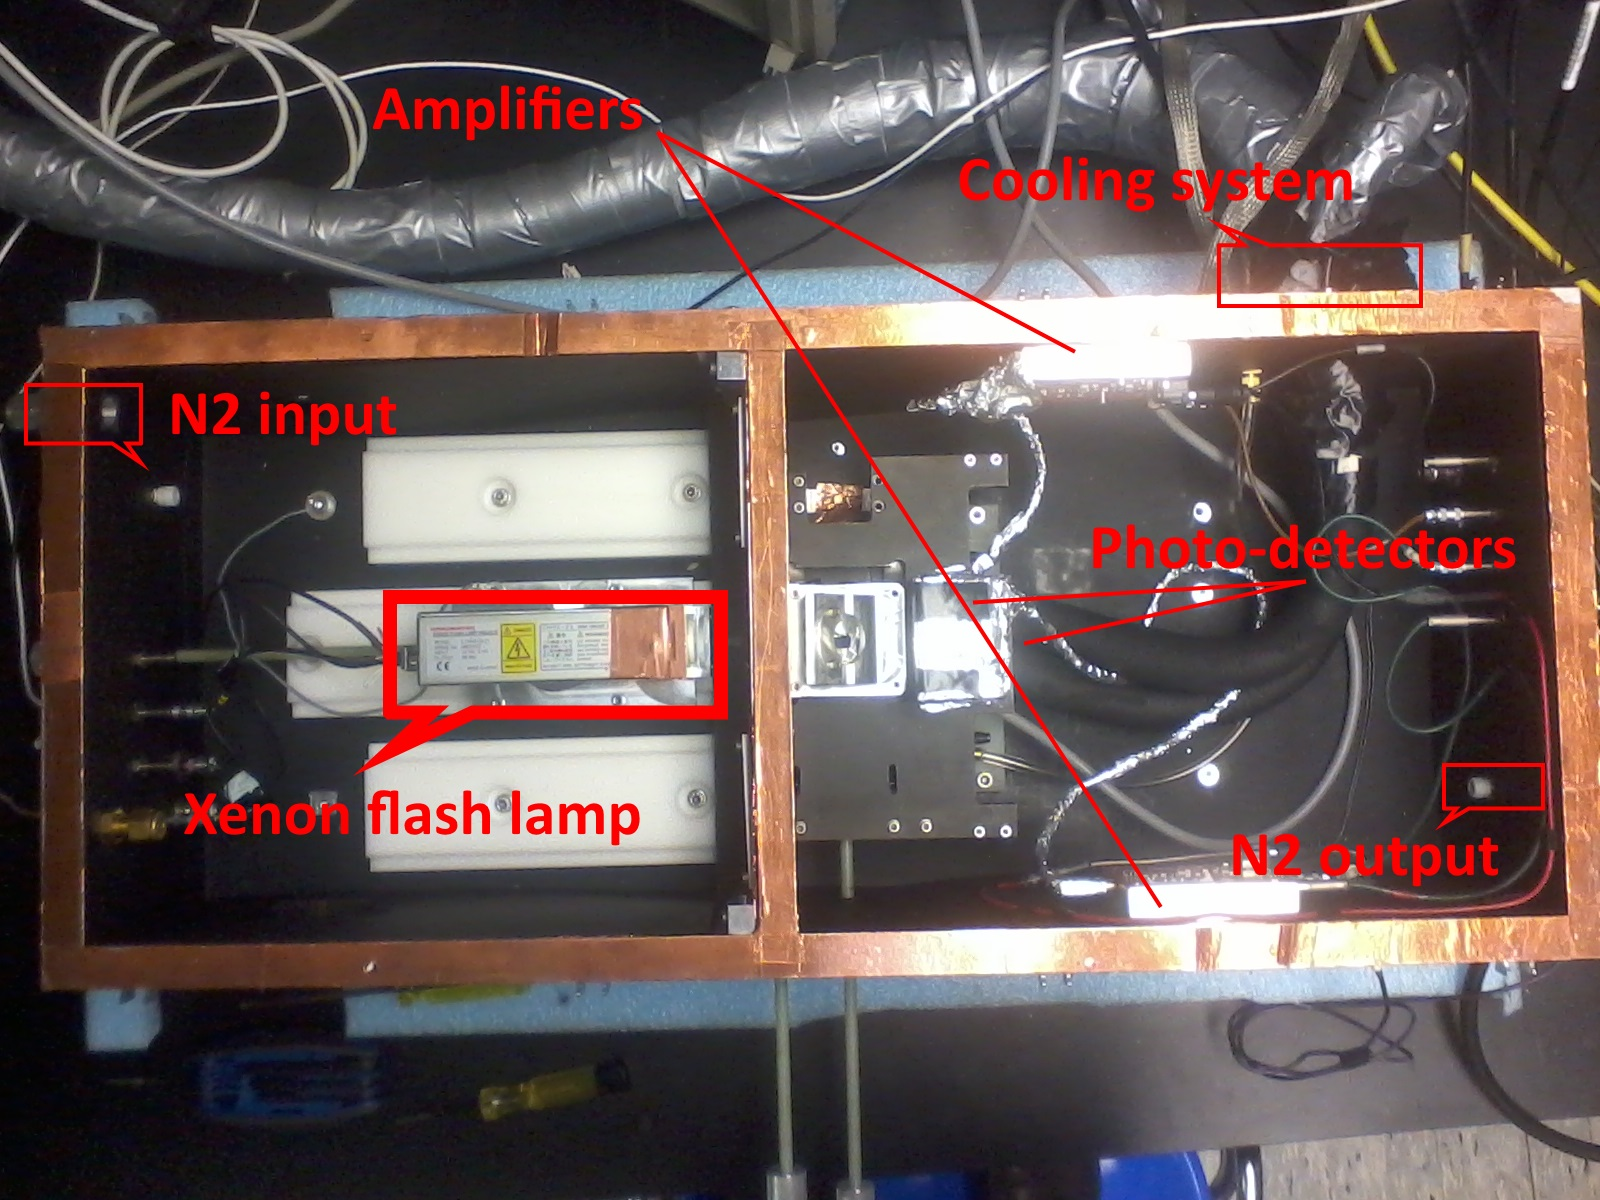
\includegraphics[totalheight=.35\textwidth,trim=0cm 7cm 0cm 2.5cm, clip=true,]{../Pictures/blabla/box.jpg}%trim=10cm 4cm 1cm 12cm, clip=true, 
    \caption{A SiPM from HAMMAMATSU VUV sensitive.}
    \label{fig:SiPM}
  \end{subfigure}%
  \begin{subfigure}{.5\textwidth}
    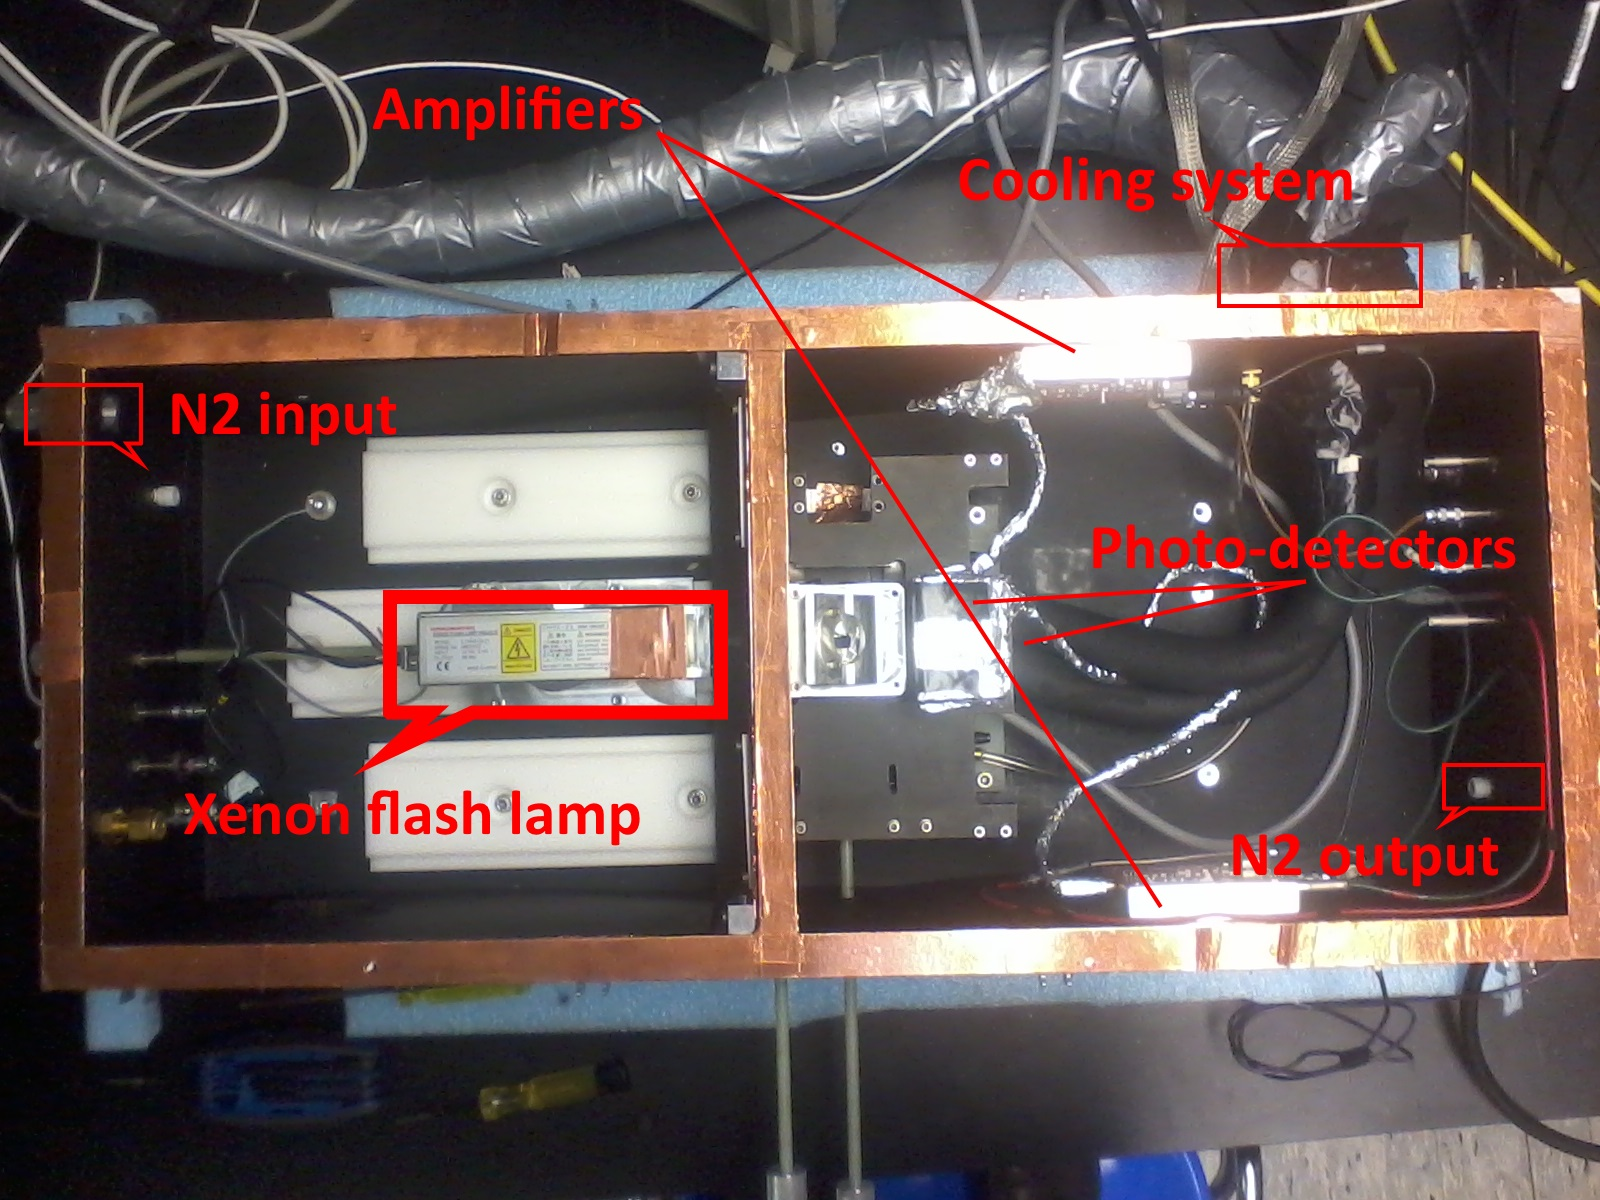
\includegraphics[totalheight=.35\textwidth,trim=0cm 7cm 0cm 2.5cm, clip=true,]{../Pictures/blabla/box.jpg}
    \caption{Equivalent circuit.}
    \label{fig:electrical_circuit}
  \end{subfigure}
  \end{figure}

  %global electrical circuit with amplifier and scope? 
  \subsection{Basic operation}\label{basic operation}
  
  Each pixel in a SiPM outputs a pulse at the same amplitude when it detects a photon. 
  A pulse produced from one pixel do not vary with the number of incident photons firing that pixel. 
  All pixels are connected to the same output channel. The total output signal is equal to the sum of those from the indidividual pixels 
  firing by photons.
  \\
  
  For example,if four photons are incident on different pixels and detected at the same time, then the SiPM outputs a signal whose ampli-
  tude equals the height of the four superimposed pulses.

  %So the number of output pulses is always one regardless the number of incoming photon. This means that MPPC output linearity gets worse 
  %as more photons are incident on the MPPC such as when two or more photons enter one pixel. This makes it essential to select an MPPC 
  %having enough pixels to match the number of incident photons.
 
  One feature of the SiPM is that each APDs operate in Geiger mode.
  
  \subsection{Physical APD's operation.}
  
  \subsubsection{PN Junction}
  A pixel is a photodiode and a photodiode has the structure of a PN junction \ref{biblio} :
  
  \begin{figure}[!hbtp]
  \centering
  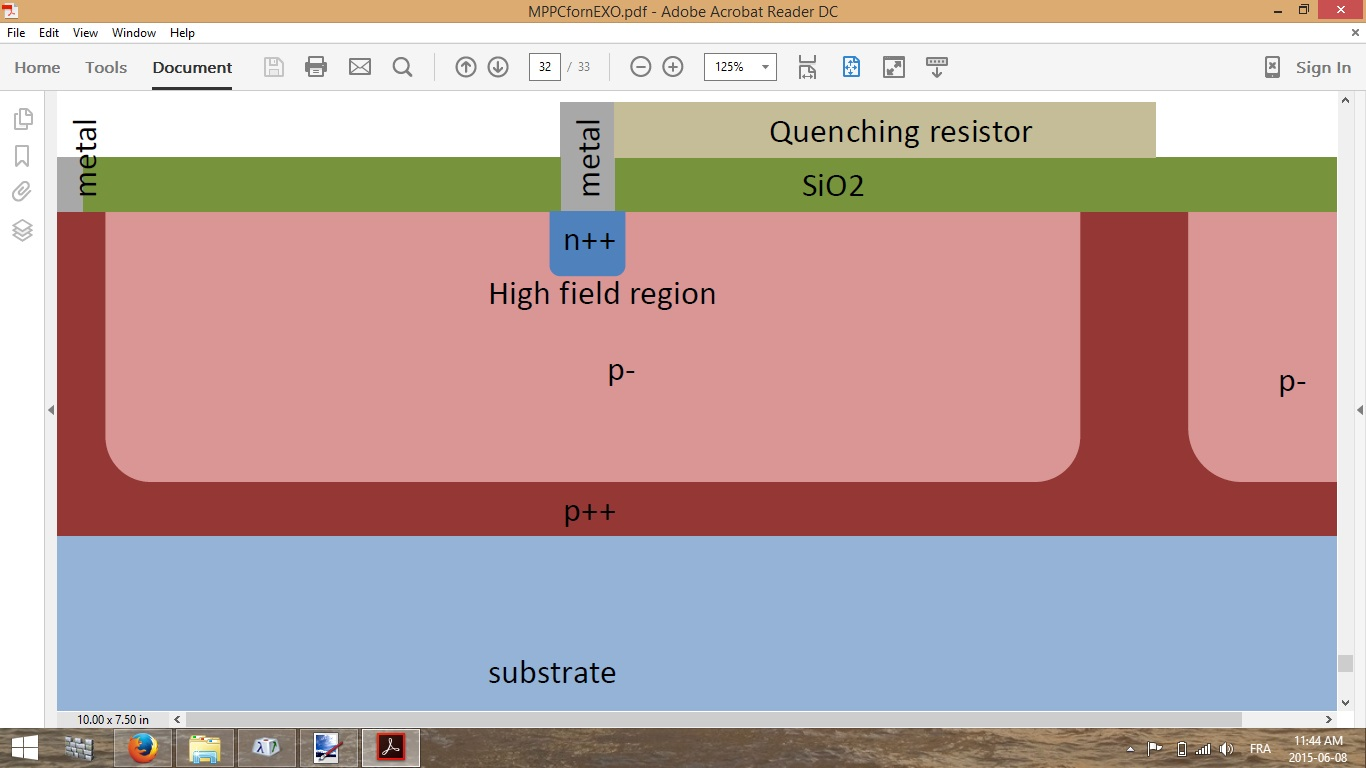
\includegraphics[trim=1.5cm 2cm 5.5cm 3cm, clip=true,totalheight=.4\textwidth]{Pictures/blabla/PN_junction.jpg}%trim=10cm 4cm 1cm 12cm, clip=true, 
  \caption{Details of a pixel of a SiPM.}
  \label{fig:PN_junction}
  \end{figure}
  
  This reference could remind the reader how works a PN junction.
  
  \subsubsection{Principe of avalanche multplication}
  
  The principle of an APD is based on the conversion of the energy of photon into free charge carriers (electrons and 
  holes)in the 
  and their further multiplication via the process of the impact ionisation. 
  \\
  When light (photon) enters a photodiode, electron-hole pairs are generated if 
  the light energy is higher than the band gap energy. Light energy (electron-volt (ev)) and wavelenght lambda (nm)
  are in relationship as shown in equation (number) below. 
  
  \begin{equation}
   e= 123/lamba
  \end{equation}
  
  A reverse volatge (or bias voltage) is applied to each opposite sides (cathode and anode) of a PN junction. The reverse voltage applied on that PN junction
  is higher than the Breakdwon Voltage (BV) of that 
  APD: this is the Geiger mode\footnote{by opposition to the normal mode where the voltage applied to a PN junction is 
  lower than the breakdown voltage}. 
  Also this reverse voltage create an electric field developped across the PN junction.\\
  When an electron-hole pair is generated in the depletion layer of a photodiode 
  the electrons (negative charge) drift towards the N+ (where the anode is) side while the holes drift towards the P+(where the cathode is)
  side due to the electric field. 
  \\
  
  The drift speed of these electron-pairs or carriers depends on the electric field strength. To a certain speed
  the carriers collide with the atoms (called crystal lattice) of the structure. But if the reverse voltage is increased even further, 
  some of the carriers which escaped primary collision with the crystal lattice will have a great energy.\\
  When they collide later with the crystal lattice, they wil generate other electron-hole pairs. This physical phenomen is called ionization:
  an electron or a hoole with high cinetical energy ionize the matter by triggering other electron-hole pairs. 
  By the end an avalanche phenomena is observed inside the avalanche region of a PN junction:
  
  \centering
  \begin{figure}[!hbtp]  
    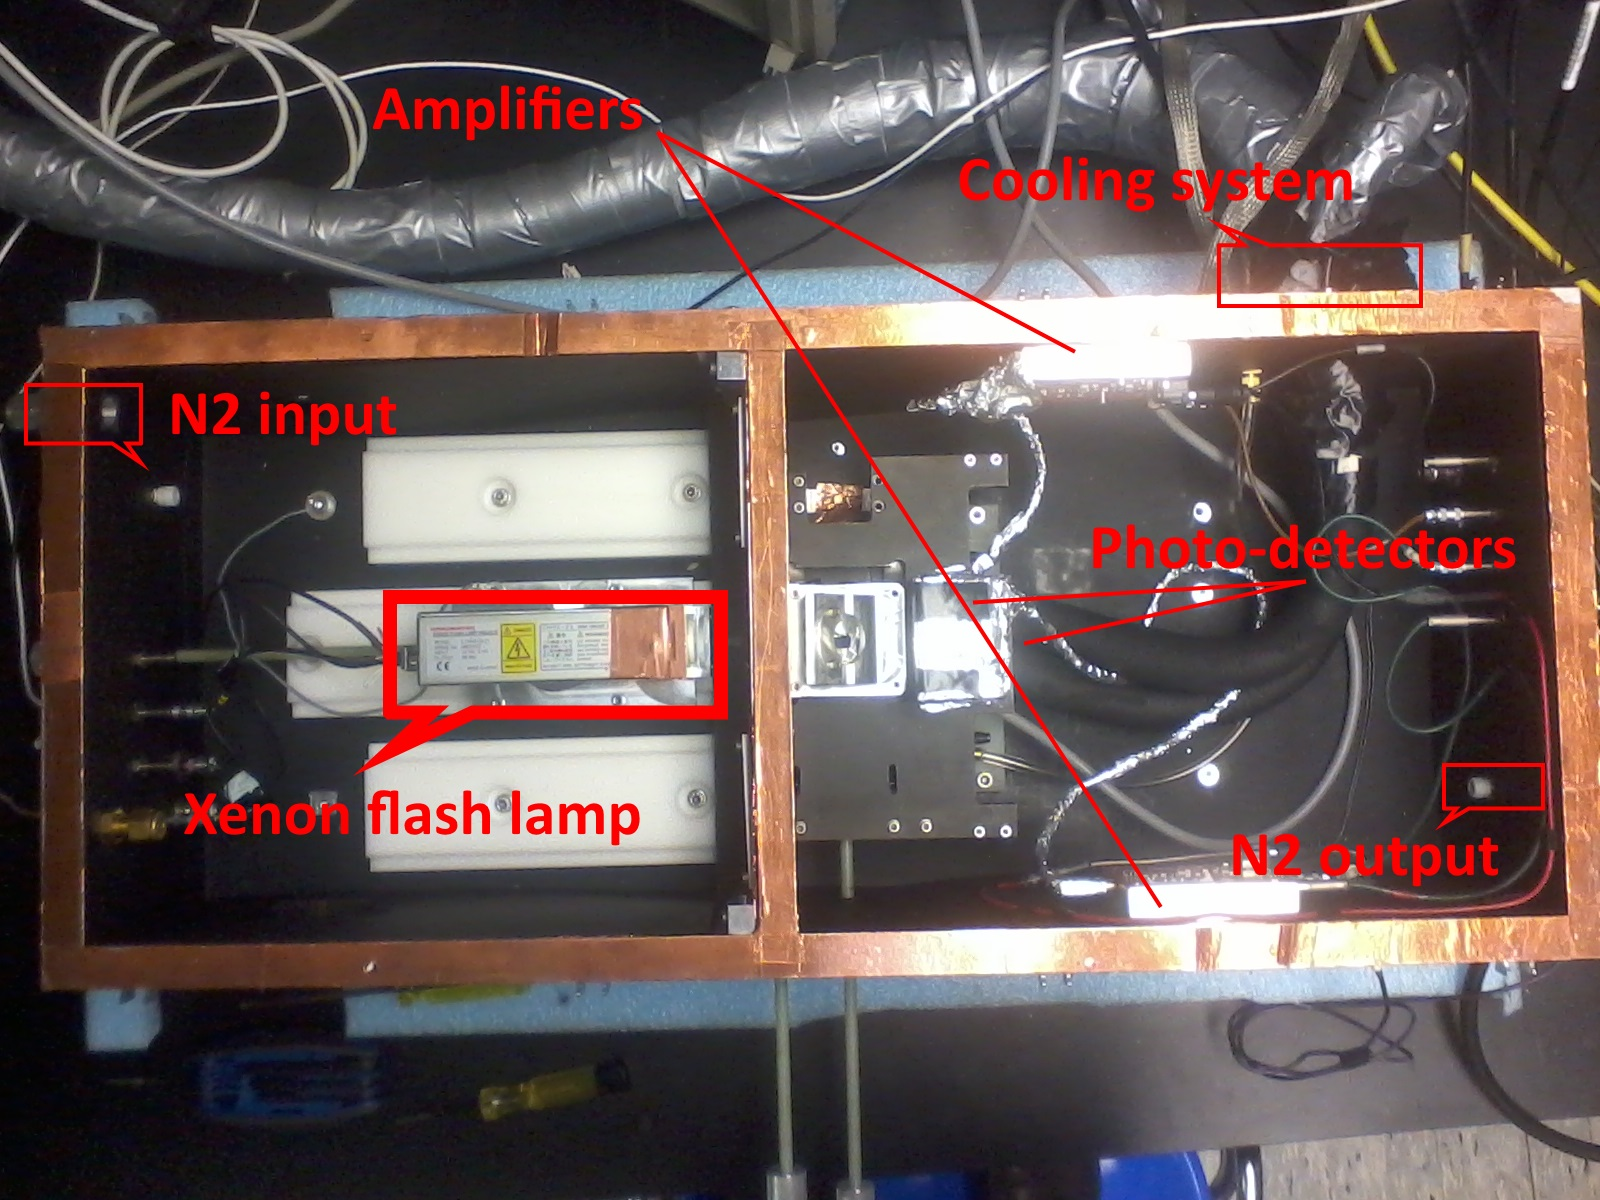
\includegraphics[totalheight=.35\textwidth,trim=0cm 7cm 0cm 2.5cm, clip=true,]{../Pictures/blabla/box.jpg}
    \caption{A photon triggers an avalanche of electron-hole pairs inside the PN junction.}
    \label{fig:avalanche}
  \end{figure}
  
  The electrons of that avalanche phenomena are collected on the anode. The resulting current is used to plot the  pluse shape. 
  To control the avalanche and so the corresponding current, a resistor is set in serie with an PN junction\footnote{The avalanche 
  is limited by the buildup of a limiting space charge in the depletion layer (p-) which decreases the field.}. 
  When the avalanche current flows through the resistor, the bias voltage applied to the junction drops below the breakdown voltage. 
  This quenches the avalanche; thus, the current decreases to zero, and the reverse voltage across the PN junction increases again above 
  its BV.
  \\
  
  The pixel is then ready to detect the arrival of a new photon.\\
  The avalanche current gives a pulse shape obeserved on the screen of an oscilloscope\ref{fig}.
  
  
  %about the gain, simple approximation speak about it ???? not now but in the gain stuff inside the corpus if room therwise in the 
  %appendix
  %Gain: The gain of the SiPM determines the charge which is produced by a single avalanche.
  %In good approximation, the gain depends linearly on the pixel capacitance C pixel and the
  %applied over-voltage V over which is defined as the difference of the bias voltage and the
  %breakdown voltage:
  %C pixel
  %C pixel
  %G = ·V over =   · (V bias −V break ).  (2.1)  q e  q e
  %Here, q e is the elementary charge and C pixel the pixel capacitance.

  \subsection{The three issues of operating SiPM.} 
  
  Such ideal picture is strongly modified by the occurrence of phenomena leading to dark current, afterpulsing effects and crootalk: 
  
  \begin{figure}[!hbtp]
  \centering
  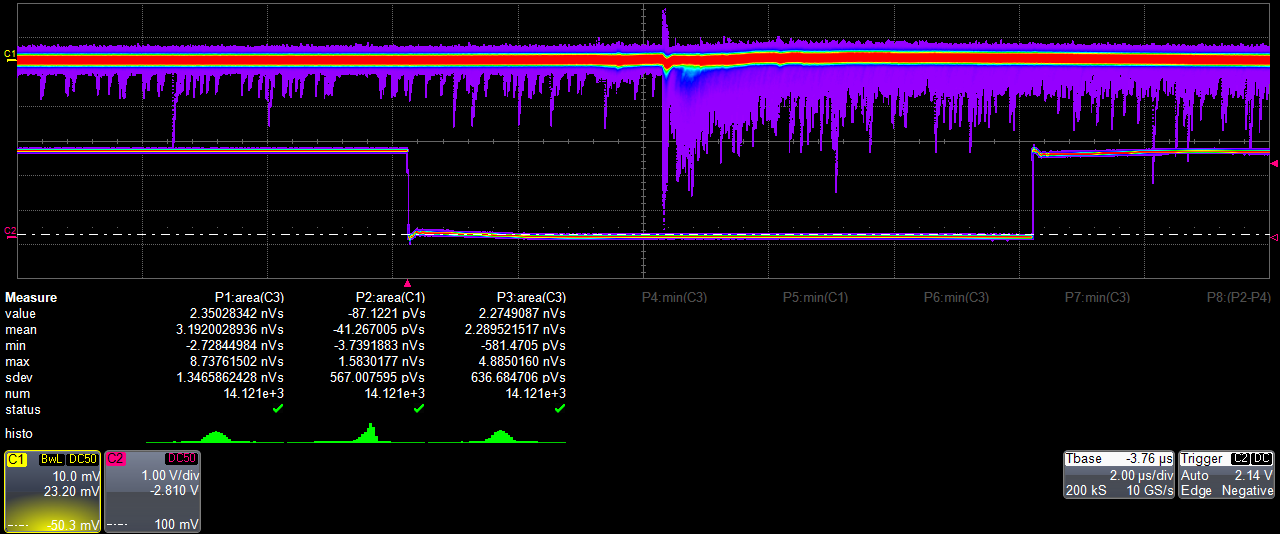
\includegraphics[totalheight=0.22\textwidth,trim=0cm 6.5cm 0cm 0cm, clip=true]{Pictures/blabla/DN_AP_CT_1.png}
  \caption{Dark noise, after-pulse and croos-talk}
  \label{fig:DN_AP_CT}
  \end{figure}
  
  \subsubsection{Dark Noise.}
  
  One of the main source of noise limiting APDs' performance is the dark noise rate.\\
  Elctron-hole pairs are generated thermally in the depletion layer. Due the reversed bias voltage applied on the PN junction, 
  the avalanche phenomena occurs.
  Unfortunately it is not possible to make the difference between avalanche triggered by a photon and avalanche triggered by hot carriers.
  The figure below prove/shows that evidence:
  
  \begin{figure}[!hbtp]
  \centering
  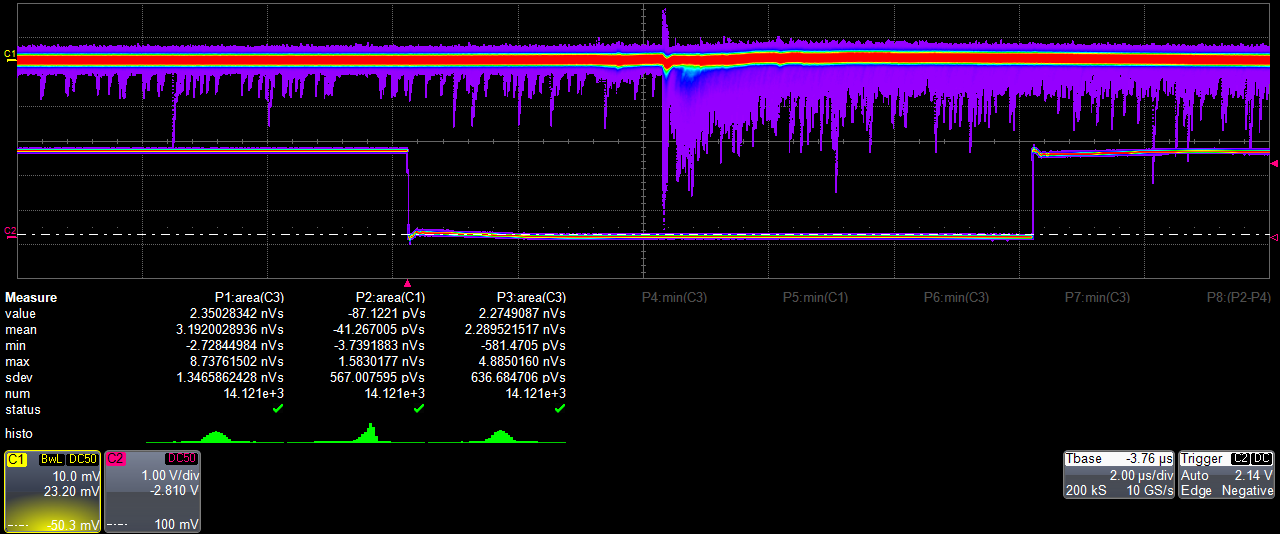
\includegraphics[totalheight=0.22\textwidth,trim=0cm 6.5cm 0cm 0cm, clip=true]{Pictures/blabla/DN_AP_CT_1.png}
  \caption{Pulse shape due to a photon is exactly the same than pulse shape dur to hot carriers.}
  \label{fig:DN_photon}
  \end{figure}
  
  Dark noise depends only of the structure of the SiPM. The array \ref{appendix} shows that HAMMAMASTU can build SiPM with low dark noise rate. 
  Nevertheless it is possible to decrease the dark noise rate by cooling down the SiPM since darke noise is generated by 
  hot carriers.  
  
  Moreover Dark noise follow a poisson law (to complete).  
  
  \subsubsection{Trapping phenomena: Afterpulsing.}

  Traps may result from damage caused by an implantation of some impurities in the fabrication process. In the depletion layer, 
  deep levels trap some avalanche carriers and release them with 
  a statistical delay. If the delay is greater than the dead time after the previous avalanche pulse, a released carrier can
  re-trigger an avalanche and cause a statistically correlated pulse. These delayed corrolated pulses are known as afterpulse. 
  \\
  
  \begin{figure}[!hbtp]
  \centering
  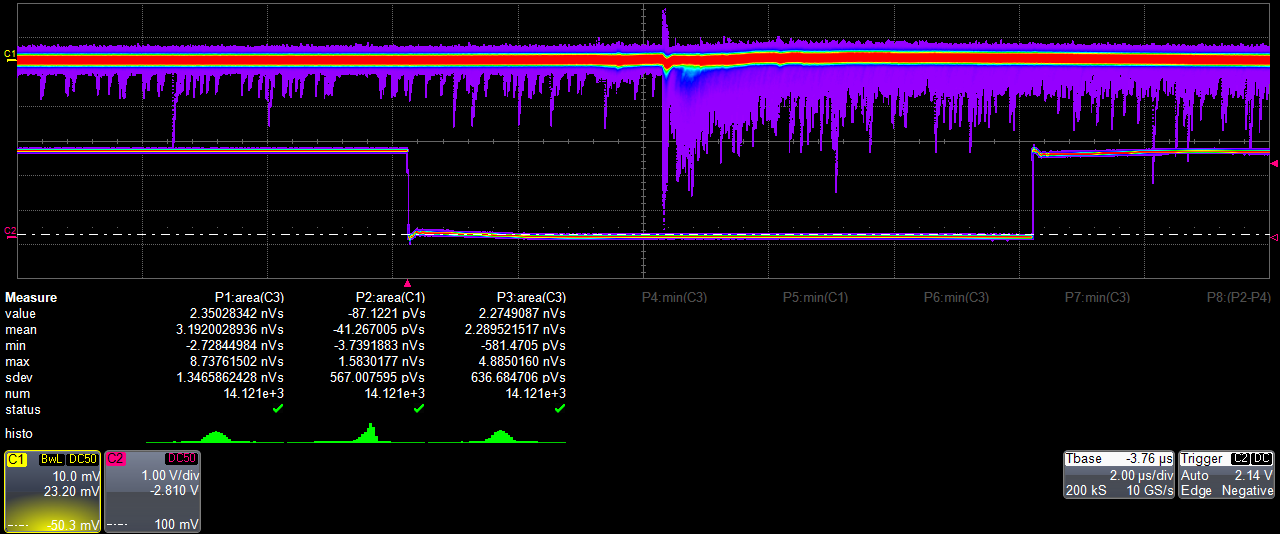
\includegraphics[totalheight=0.22\textwidth,trim=0cm 6.5cm 0cm 0cm, clip=true]{Pictures/blabla/DN_AP_CT_1.png}
  \caption{After pulses are clearly identified with the persistent mode of the oscilloscope.}
  \label{fig:AP}
  \end{figure}
  
  The probability that an afterpulse occurs increases with the reversed bias voltage applied on the SIPM.  A solution to diminish 
  significatively afterpulse effects is 
  to operate at low reversed bias voltage, but at the expense of degrading the photon-detection efficiency (see section). 
    
  After pulse follow a law. 
  
  \subsubsection{Optical crosstalk.}
  
  Hot carriers (e.g., dark noise) in avalanche PN junction has a certain probability to emit photons with energy higher than 1.14 ev (higher than 
  the band gap energy described in section).\\
  Depending on their energy and the location where they are produced, these photons have a certain probability to reach a 
  neighbouring pixel and to produce an additional avalanche. 
  
  \begin{figure}[!hbtp]
  \centering
  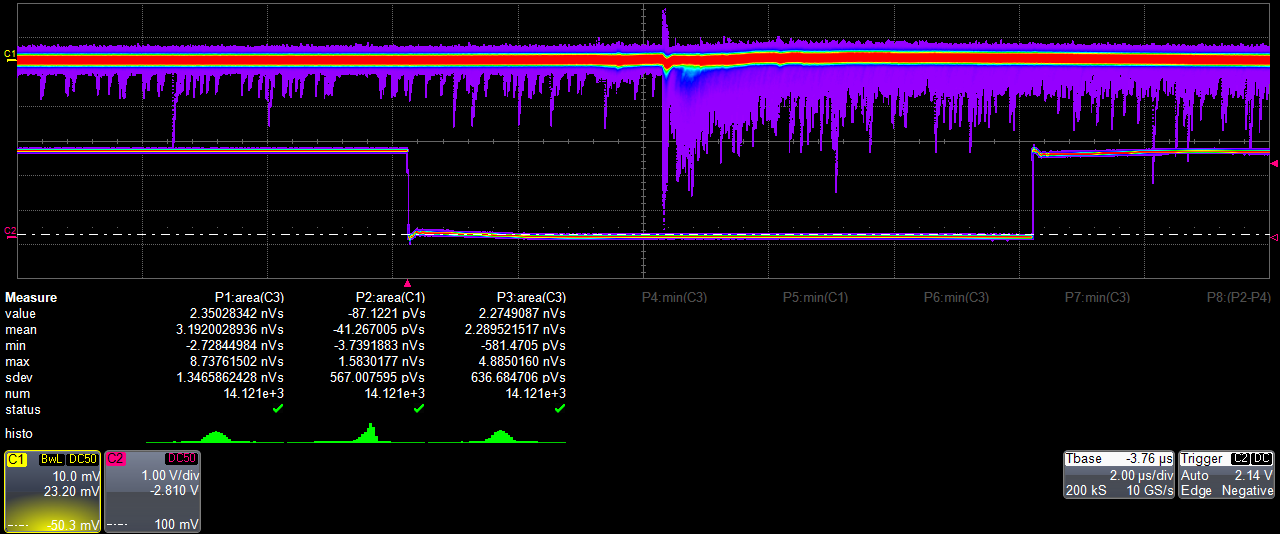
\includegraphics[totalheight=0.22\textwidth,trim=0cm 6.5cm 0cm 0cm, clip=true]{Pictures/blabla/DN_AP_CT_1.png}
  \caption{Photons emit may reach a neighbouring pixel and trigger there an avalanche.}
  \label{fig:CT}
  \end{figure}
  
  So at conditions where only one pixel is expected to be excited simultaneously than its neighbouring pixels, crosstalk results in output 
  pulses with amplitudes twice or several times the amplitude of a single triggered pixel
  \footnote{The section\label{Basic operation} reminds that ``The total output signal is equal to the sum of those from the indidividual 
  pixels firing by photons''.}
  
  A technical solution is to build an optical wall between two pixels (not enough). 
  \\
  
  The probability of observing crosstalk is proportional to the SiPM gain and so to the reversed bias voltage. The same conclusion about the 
  efficiency made in the previous subsection are obeserved for crosstalk. 
  
  The law
  
  
  \section{Encountered issues}  
  
  Before recording waveforms and analysing them I dealed with some issues but mainly with electronic noise.\\
  Light leaks appeared when the \xfl was operating. They can hinder and negate the results of data collection. 
  Two kinds of light leaks have been observed :
  
  \begin{itemize}
   \item Visible light leaks.
   \item Radiofrequency light leaks.   
  \end{itemize}
  
  \subsection{Visible light leaks}
  
  Visble light leaks come from outside of the box or from the \xfl (If ... complete).\\
  This phenomena has mainly an impact on the dark noise rate and on the calculation of the efficiency.
  To avoid visible light from the \xfl, the last one is covered with black box. Also to absorbe photons from such visible light
  walls and lid is covered by matt black absorbing vin.\\
  To avoid light from outside of the box, the whole box was covered with a black tissue. The section \ref{} shows how we check if some
  visible light from outside could reach detectors inside the box. 
  
  \begin{figure}[!hbtp]
  \centering
  \begin{subfigure}{.5\textwidth}
    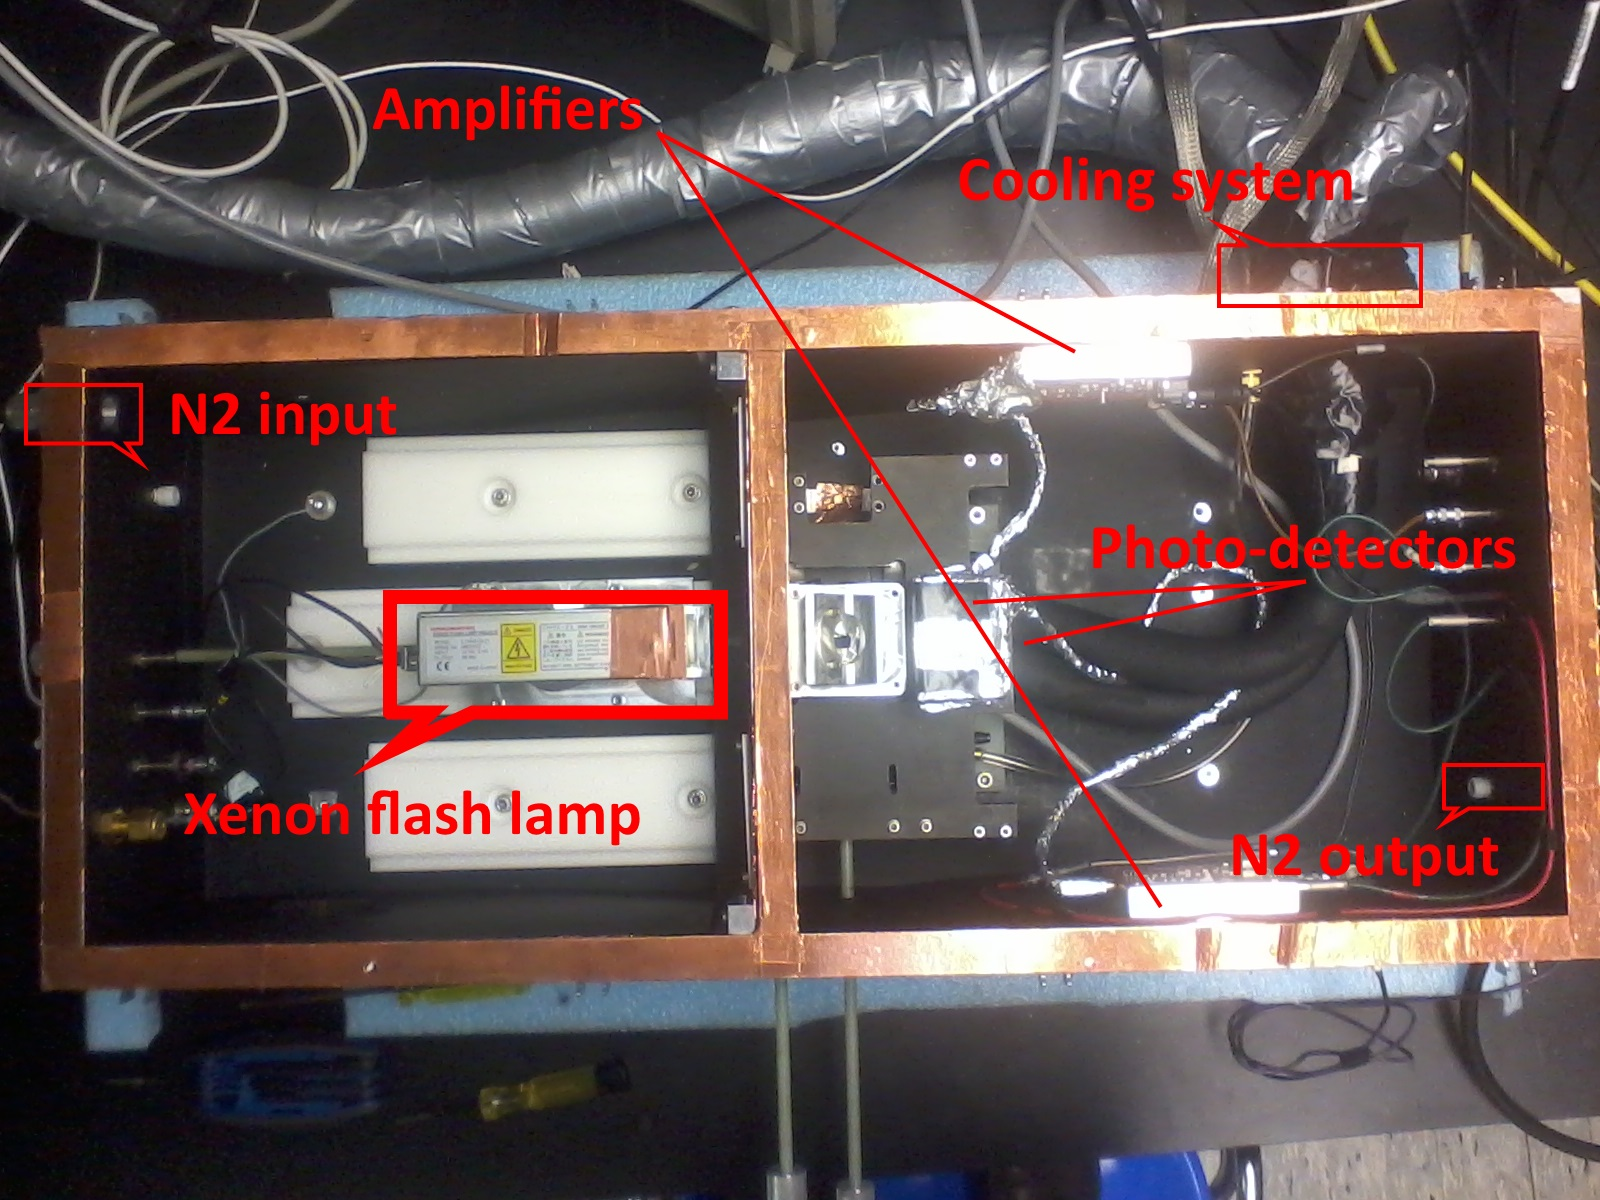
\includegraphics[totalheight=.35\textwidth,trim=0cm 7cm 0cm 2.5cm, clip=true,]{../Pictures/blabla/box.jpg}%trim=10cm 4cm 1cm 12cm, clip=true, 
    \caption{A SiPM from HAMMAMATSU VUV sensitive.}
    \label{fig:SiPM}
  \end{subfigure}%
  \begin{subfigure}{.5\textwidth}
    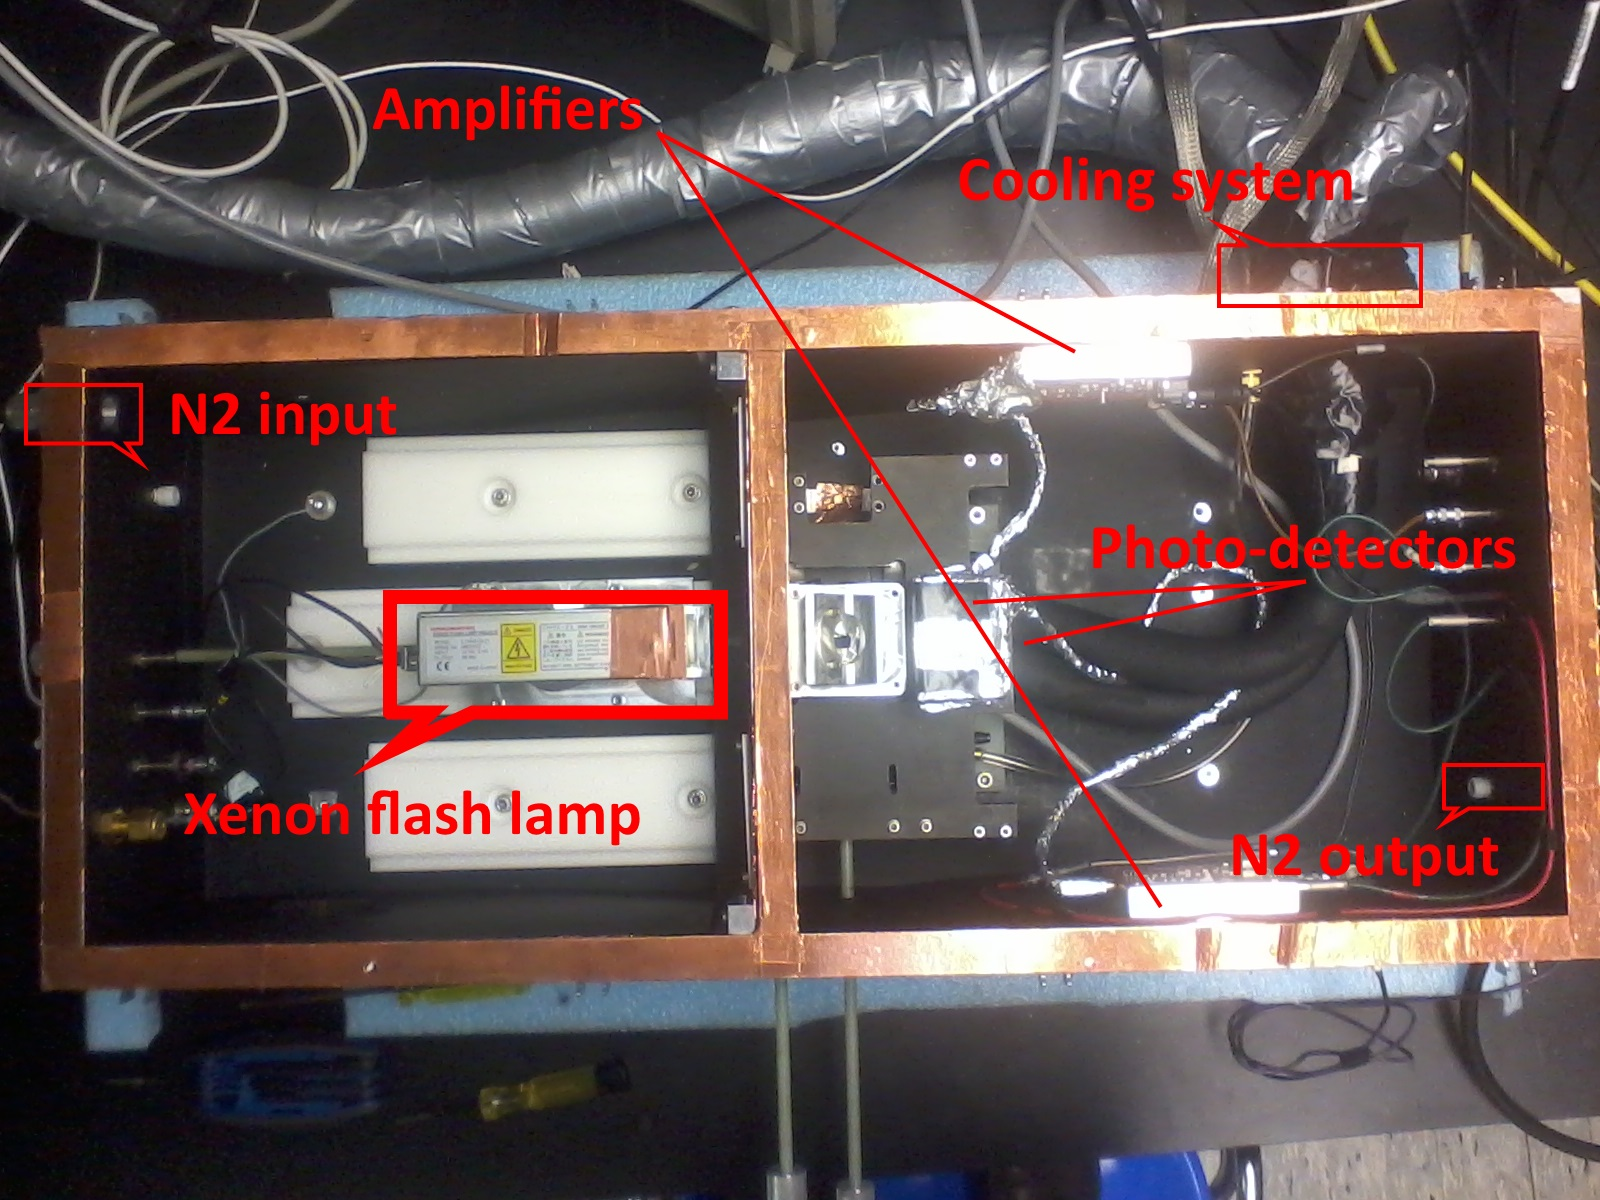
\includegraphics[totalheight=.35\textwidth,trim=0cm 7cm 0cm 2.5cm, clip=true,]{../Pictures/blabla/box.jpg}
    \caption{Equivalent circuit.}
    \label{fig:electrical_circuit}
  \end{subfigure}
  \end{figure}
  
  \subsection{Radiofrequency light leaks.}
  
  Radio frequency light leaks result in electromagnetic noise on the signals from the detectors.\\  
  Radiofrequency noise occured when the \xfl was triggered by a square wave pulse generator. Too much readiofrequency noise disturbed 
  the signals of the photodetectors. The figure \ref{} shows clearly that electronic noise covers, deformes or amplifies pulse shapes.
  
  \begin{figure}[!hbtp]
  \centering
    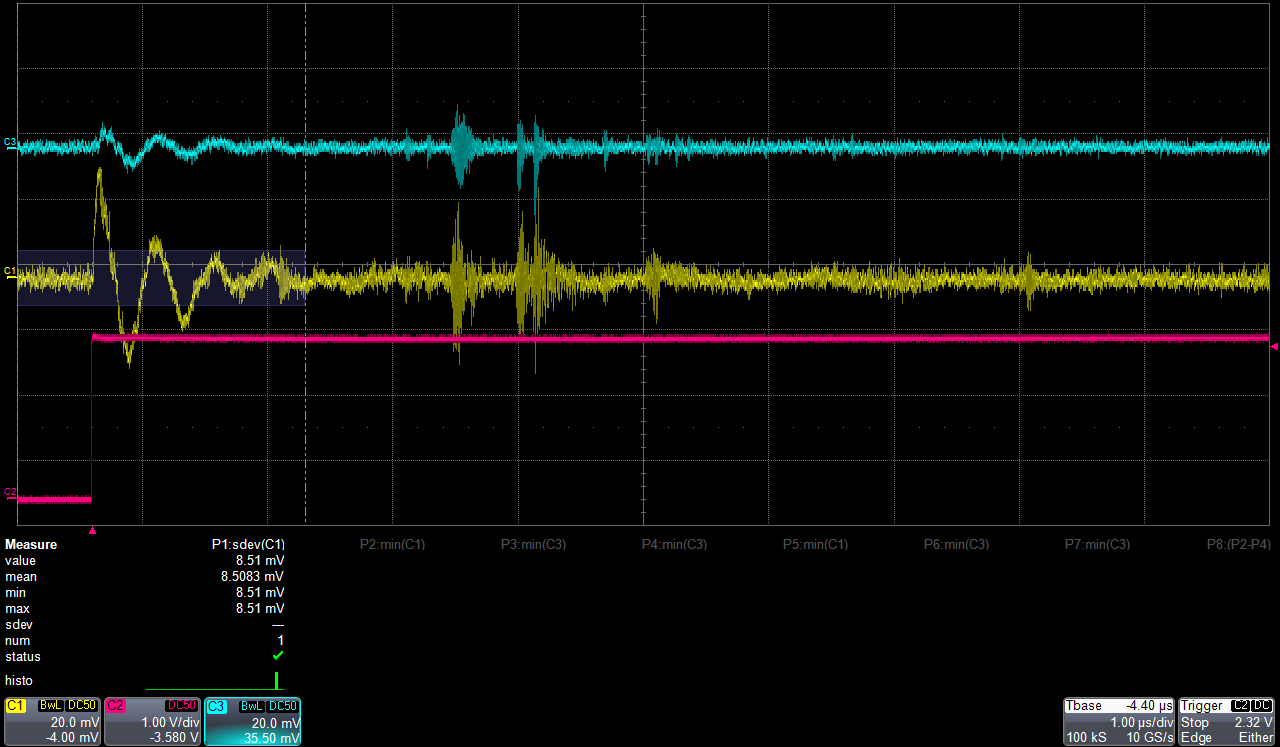
\includegraphics[totalheight=0.4\textwidth,trim=0cm 5.5cm 0cm 0cm, clip=true]{Pictures/lamp_noise_apr17_2.png}
  \label{fig:noise_signal}
  \end{figure}
  
  \subsubsection{Sources of electromagnetic noise.}
  
  We noticed that electronic noise came from electromagnetic sources. So

  \begin{itemize}
  \item Some devices were not grounded. The signal from the photodetector oscillate\ref{fig:noise_signal}
  ~\ref{fig:signal_with_noise}.
  \item When the \xfl was working it was creating some radio waves propagating through the air and which were then transmitted to any piece of conductive metal of the 
  box. The consequences were : 
    \begin{itemize}
    \item The aluminium lid of the box conducted everywhere the electric field of these radio waves, which disturbed the amplifiers.
    \item Each detector could feel these radio waves and the signal got worst.
    \item The metal divider acted as a transmitter and the piece of metal of the signal wires connected to the amplifiers acted as antenna.
    \end{itemize}
  \end{itemize}
  
  \subsubsection{Three main solutions.}
  
  The first solution was to create a ground point on which all devices - especially the square wave pulse generator - were connected with the same wire 
  (to avoid ground loops). In that way, the oscillations of ~\ref{fig:comparaison} were removed. 
  
  \paragraph{\underline{\emph{Isolate the lid from the box.}}}
  
  As it was described above, the electric field from the radio waves propagates through the entire lid. When the box was closed it disturbed the working 
  amplifiers. The solution was to isolate the lid from the box by adding black tape and to guide the electric field with copper on the edge of the lid
  to the ground point.

  \paragraph{\underline{\emph{Isolate the \xfl.}}}
  
  As the \xfl creates radio waves, we decided to isolate it by building a faraday cage around it. We added a thick piece of metal to absorb radio waves 
  and we covered this first part of the box with aluminium foil. In that way the electric field propagates through the aluminium foil to the edge of the top
  box to the ground point. 

  \paragraph{\underline{\emph{Isolate the photo-detectors and the amplifiers.}}}
  
  As the bottom and the top detector seems to capture radio waves, two faraday cages were created to protect them.
  
  This picture below could summarize our work (yellow signal is the bottom photodetector and the blue one is on the top):
 
  \begin{figure}[!hbtp]
  \begin{minipage}[t,High electronic noise level.]{0.49\linewidth}
    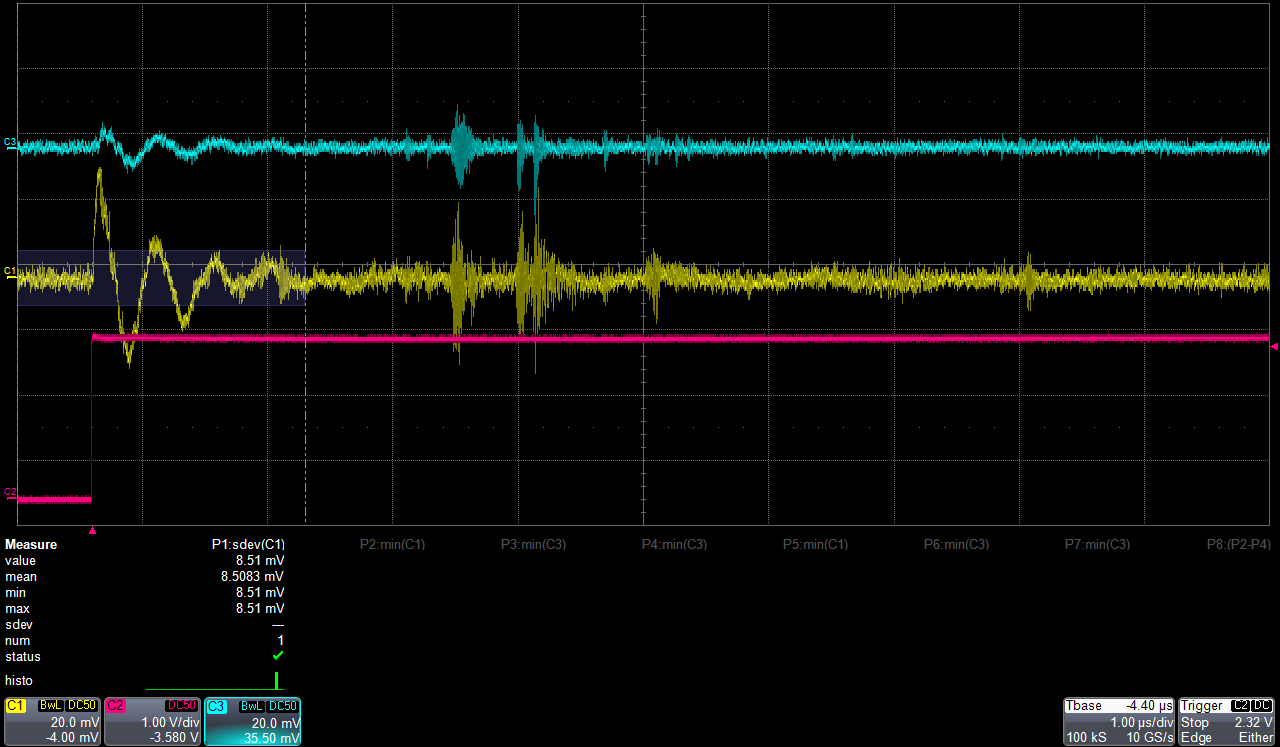
\includegraphics[totalheight=0.4\textwidth,trim=0cm 5.5cm 0cm 0cm, clip=true]{Pictures/lamp_noise_apr17_2.png}
    %\centering{\caption{Noisy signals.}}
    %\label{fig:Noisy_signals}
  \end{minipage}
  \quad
  \begin{minipage}[t,Low electronic noise level.]{0.49\linewidth}
    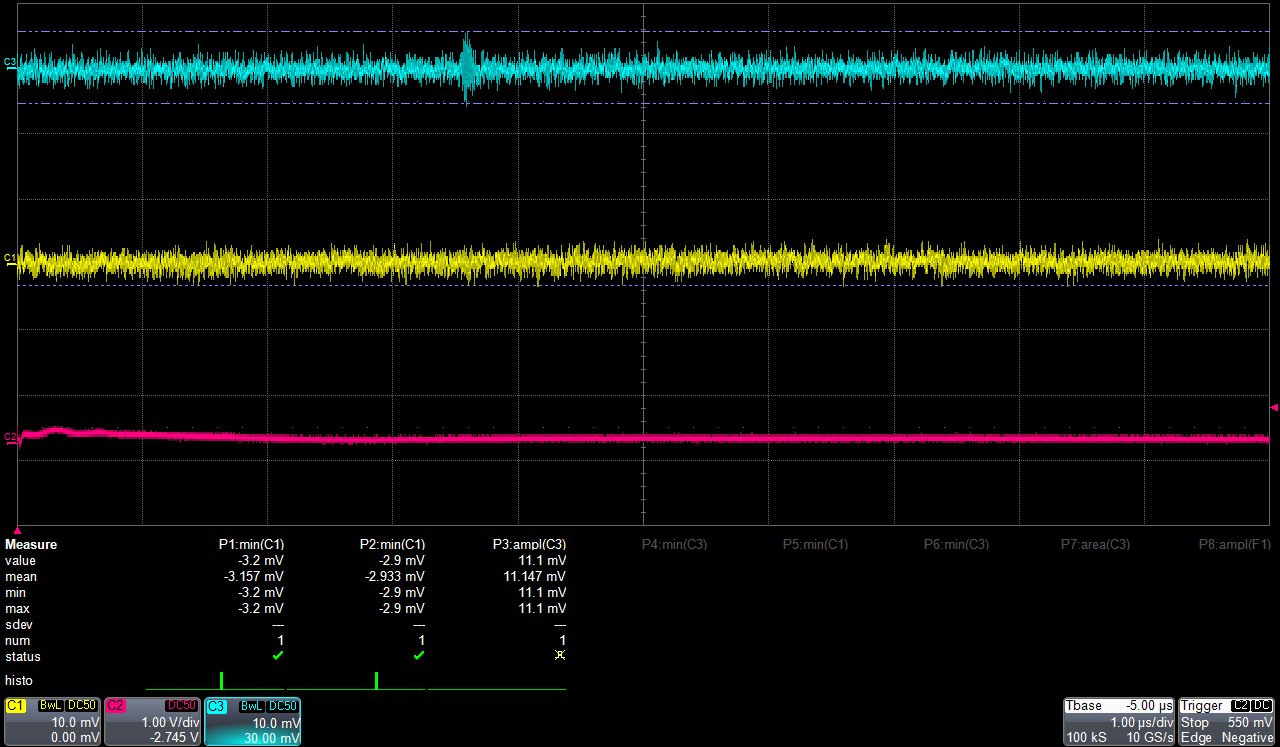
\includegraphics[totalheight=0.4\textwidth,trim=0cm 5.5cm 0cm 0cm, clip=true]{Pictures/good_elec_noise.png}
    %\centering{\caption{The electronic noisehas dispeared.}}
    %\label{fig:good_signals}
  \end{minipage}
  \caption{The noise level before (left) and after (right) solving the issues.}
  \label{fig:comparaison}
  \end{figure}
  
  
  %\begin{figure}[!hbtp]{0.49\linewidth}
  %\centering
  %\subfigure[High electronic noise level.]{
  %  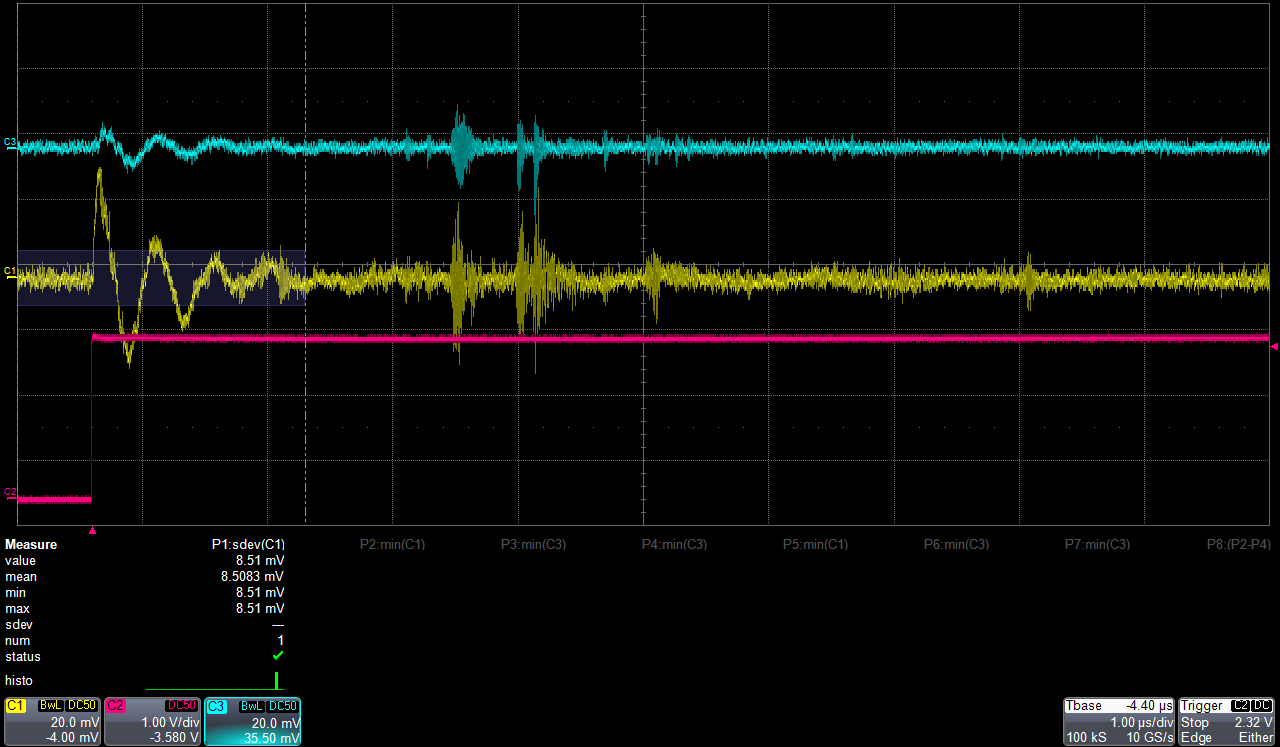
\includegraphics[totalheight=0.4\textwidth,trim=0cm 5.5cm 0cm 0cm, clip=true]{Pictures/lamp_noise_apr17_2.png}
   % \label{fig:noise_signal}}
  %\quad
  %\subfigure[Good The electronic noisehas dispeared.]{%
    %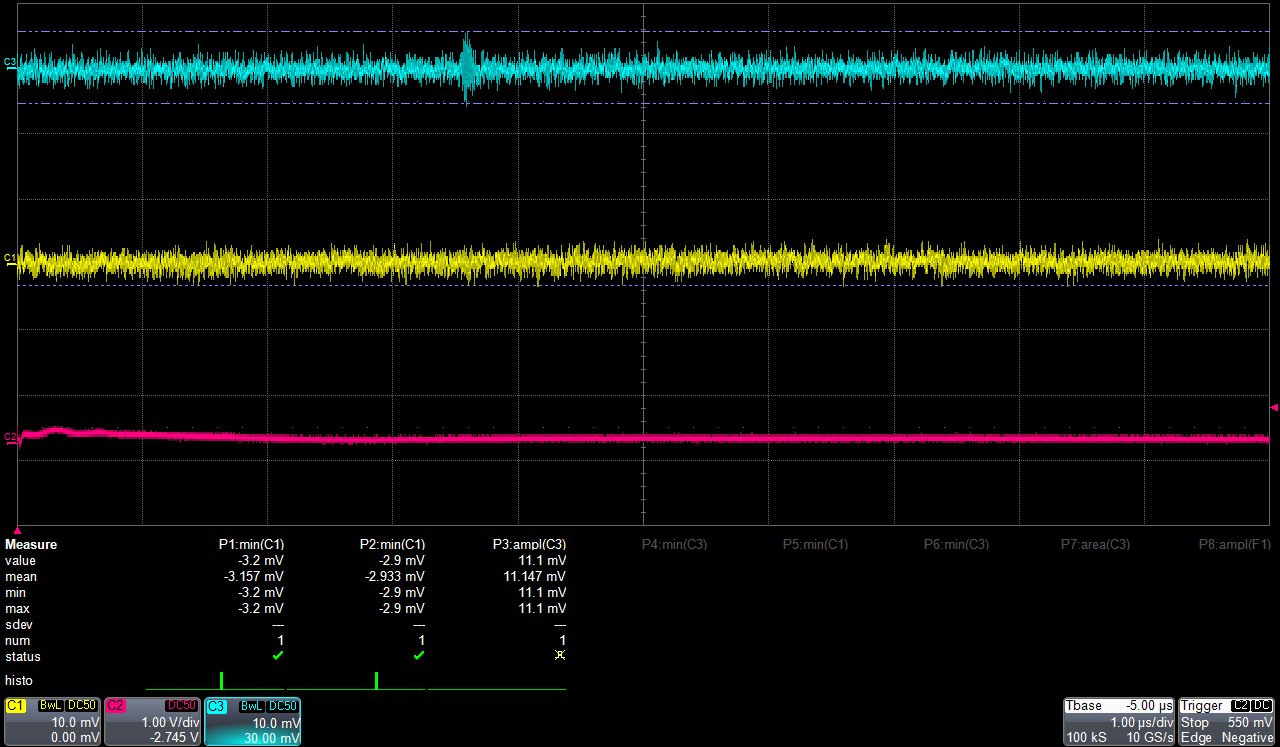
\includegraphics[totalheight=0.4\textwidth,trim=0cm 5.5cm 0cm 0cm, clip=true]{Pictures/good_elec_noise.png}
    %\label{fig:good_signal}}
 % \caption{The noise level before (left) and after (right) solving the issues.}
 % \label{fig:comparaison}
 % \end{figure}
  
  A SiPM, placed on the top, was used as a reference. It let us check if the light remained constant when we characterized a MEG MPPC and a VUV3 SiPM at 
  $-100^\circ$C.
  
  
  \section{DN rate and After Pulse}
  
  \subsection{recoveries time and amplitude/distribution of tim ..}
  
  As mentioned earlier, the distribution of the timing difference between consecutive pulses is used to measure the dark noise and 
  after-pulsing rates. The starting pulses are required to correspond to the oscilloscope trigger in order to properly
  account for the oscilloscope dead time. The starting pulses are also required to correspond to single pixel avalanches
  (i.e. triggers with cross-talk are excluded) in order to measure the after-pulsing rate generated by a single parent avalanche.
  On the other hand, the second pulse can have any amplitude (above the noise). 
  
  Fig pulse amplitude vs time newt pulse shows the amplitude of the second pulse as a function of the time difference with the trigger
  pulse. 
  The main band (the first one with fitting function) at ∼40 mV corresponds to single pixel avalanches. 
  Cross-talk yields pulses with amplitudes two, three, or more times larger. 
  
  10³ ns = 1 µs; lamp send pulse of 10 µs -> 10⁴ ns.
  
  There is no correlation between time and amplitude except below 100 ns where a drop below the 40 mV value is clearly visible. 
  Physically inside the  photodector, after an avalanche the voltage across the diode indeed recovers with a time constant 
  given by the product of the pixel capacitance and quenching resistance. The pulses that do not have lower amplitude even
  though they occurred within the recovery time scale must
  come from different pixels. It is likely that these pulses are
  delayed cross-talk, the seed charge carrier being created by
  photons from the parent avalanche subsequently diffusing to
  a neighboring pixel. This feature is also clearly visible for the VUV3. 
  
  The timing distributions are shown in Fig. 15 including the function that best fits the data. Each step on a log-log plot
  corresponds to a distinct exponential time dependence. The last step corresponds to distribution of dark pulses. It is clearly
  visible for all 3 devices. 
  
  The difference is striking because the FBK-2013 SiPMs are 9 times smaller in area than the VUV3. check this for our experience. 
  
  dark noise rate is an order of magnitude too high
  
  after pulse : After-pulsing rates were also extracted by fitting the distributions
  the total after-pulsing rate and the after-pulsing rate within the first 10 μs that is relevant for our application
  exceeds the specification of 20% for the combined rate of cross-talk and after-pulsing. 
  
  expect limit the number of correlated pulses (cross-talk and after pulse) to less than 0.2 per parent pulse.
  
  
  
  
  
  The darknoise rate is the signature of each device. So to know this signature let us know to compare different devices between them. 
   
  \subsection{methodology for DN and AP: theoriticl calculation and how to act on the setup}
  
  One of the main source of noise limiting the SiPM performance is the dark noise rate, which mainly originates from the electron 
  created thermally in the depletion layer (p-) \ref{figure}. These carriers trigger avalanches exactly as if the pixel would have been fired.
  \\
  To calculat the DN rate, the goal is to count the number of time the screen of the scope
  displays on pulse (by opposition at two pulse detected on the same time \ref{section}). So a simple idea is 
  to record the minimum of of pulses on the dark region \footnote{see ection/figure}. It is quiet easy to understand
  that we have to focus on the dark region only. Indeed the light region match one PE peak match with the detection of one photon-electron send from
  the lamp bu also corresond/reflect the DN/match with the detection of one PE from DN. So the light region of the scope do not let us determine for shure from where comes 
  this pulse. So to avoid to be confused we have to focuse on the dark region only. 
  \\
  
  On the scope we trigger one the lamp.then we recorded the minium of pulses of the dark region and plot
  them on an histogram. The first PE peak match with the detection of zeroPE. The second with detection of one PE etc. 
  
  \subsection{results : plot}
  
  The historgam of fig (section PE) is used for DN..
  
  nEXO experiment requires that at -100C, the DN rate should be less than 50HZ/mm². 
  It is interesting to observe tat the DN rate decrease with the temeperature. 
  
  \begin{figure}[!hbtp]
  \centering
  \includegraphics[totalheight=0.4\textwidth,trim=1.8cm 1cm 5.5cm 3cm, clip=true]{Pictures/Pictures_MEG/DN.png}
  \centering{\caption{light region.}}
  \label{fig:pulse_shape}
  \end{figure}

  
  \subsection{analyse : pont entre méthodoligie et solution }
  
  \paragraph{factor which could influence DN}
  
  The DN depends of each device. The DN depend only of the temperature as it was described above. 
  
  \paragraph{}
  
  the ref and the annexe could givemore detail about the theoritical calculation of DN. 
  
  \begin{equation}
    P_{D0} =  exp(-<DN>) \iff <DN> = -ln(P_{D0}).
  \end{equation}
  
  The DN follows the poisson law. That why in the histogram we inegrate zero pe. For a number of waveform constant/
  for the same total number of waveform, when the temperature decrease, the DN decrease. So the number pe upper than the detection
  of one PE decrease also \ref{see part below} while the number of zero pe increase. 
  According to the equation above, Po increase and so DN decrease.   
  
  \paragraphe{conclusion}
  
  Compared to the MEG SiPM, the VUV3 is a good quandidat for nEXO.  
  
  \section{CT}
  
  They unfortunately all exceed 20%, 
  which is our upper limit for the correlated avalanche probability that includes cross-talk and after-pulsing.
  
  Hot carriers in avalanche p-n junction emit photons even in the visible range \footnote{see section}. Thus, 
  during the avalanche breakdown, a photodiode operating in Geiger mode may emit a few photons. 
  The photons emitted will be detected by neighboring pixels despite an optical wall between two pixels \footnote{see picture annexe}. 
  \\
  
  It is quiet esay to identify crosstalk on the screen of the scope \footenote{see section, gif orput figure}. 
  When the height of a peak is double compare to its neighbor, this peak is a cross talk. Physically that means that two avalanche appears and end 
  on the same time : one comes from the photon coming from a neighboring pixel and the other one comes from the detection of a photon or 
  reflect dark noise. 
  
  \subsection{methodology for CT: theoriticl calculation and how to act on the setup}
  
  When we trigger on the lamp, the minium for each waveform recorded is taken in account/ is recorded. Then we construct an histogram 
  \footnote{see section} where the first peak of the histogram match with zero peak. The second peak match with the detection of a photon or 
  comes from dark noise. The third peak match with the detection of two photon on the same time, ie crosstalk.\\
  The screen on the scope displays gaussian noise for the case, a single peak for the second and a double higher peak for the third. 
  
  So to analyse crosstalk, the idea is to eradicate the first peak of our previous histogram. the goal
  is to obtain an histogram where the first peak match with the detection of 
  one photon while the second peak of this futur histogram match with the detection of two photon which appear on the 
  same time.\\
  That means that instead of triggering the scope when the lamp send flash we have to trigger when the scope displays
  one peak corresponding to the detection of one photon or coming from dark noise. 
  So as it has been seen previously\footnote{see section} that the DN is always appearing, we triggered on the detector. 
  image. 
  
  \paragraphe{method}
  1 range of time of 2ns(1ns before and 1ns after}\\
  2 set a threshold at 3.5 times the baseline to record a minimum amplitude\\
  3 Set data in a table and plot an histogram
  4 Integrate the first peak and divide by the totale number f waveform (or integrate the histogram from the beginning of the first peak)
  
   
  
  \subsection{results : plot}
  
  Here is an histogram of CT for VUV3 @ -100C. The first peak correspond to the detection of one photo-electron, 
  the second one to the detection of two photo-electron etc...
  
  \begin{figure}[!hbtp]
  \centering
  \includegraphics[totalheight=0.4\textwidth,trim=1.8cm 1cm 5.5cm 3cm, clip=true]{Pictures/Pictures_MEG/CT_histrogram.png}
  \centering{\caption{Hitogram coming from analysing crosstalk for the VUV3 SiPM @ -100C. }}
  \label{fig:CT_hitogram}
  \end{figure}
  
  The array \ref{see above} describ some device we test. The most intrinsting devices are the MEG SiPM and 
  the VUV3 SiPM both of them from Hammatsu. 
  
  \begin{figure}[!hbtp]
  \centering
  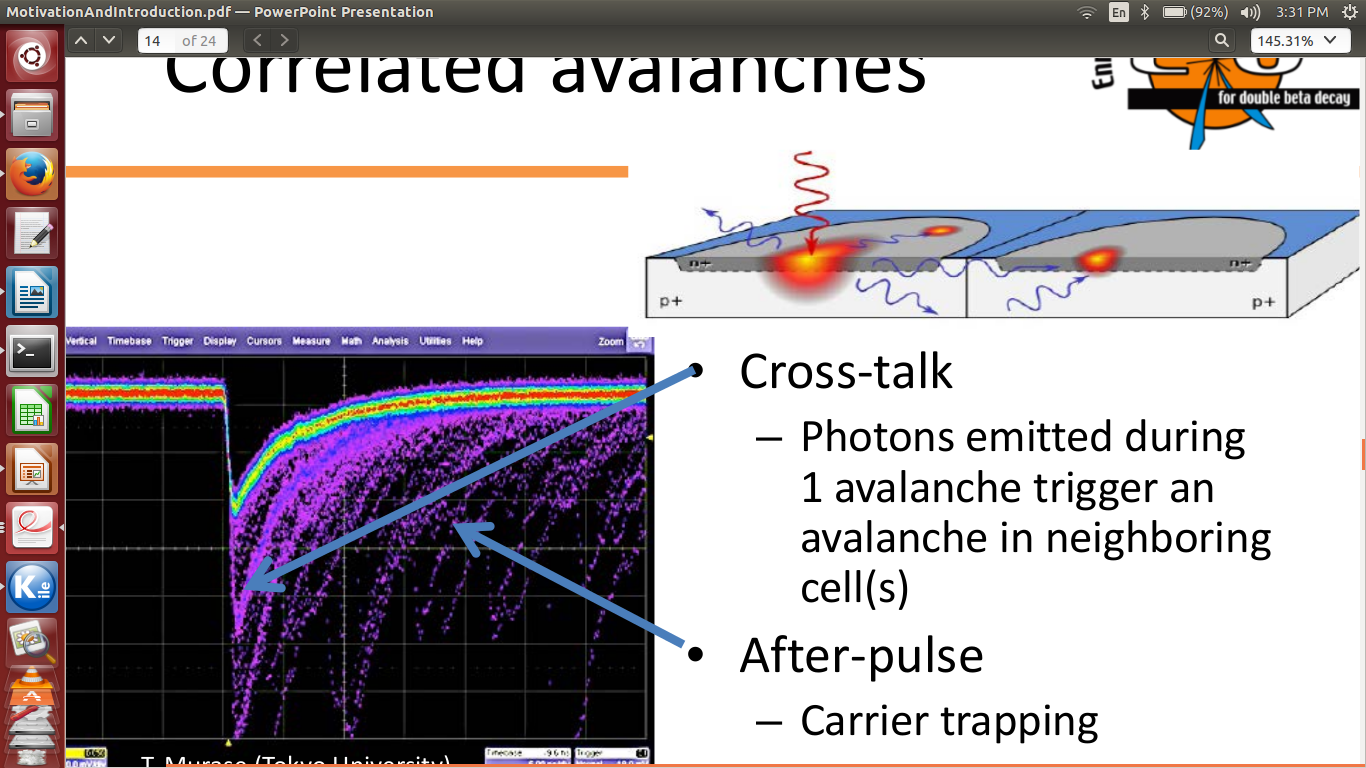
\includegraphics[totalheight=0.4\textwidth,trim=1.8cm 1cm 5.5cm 3cm, clip=true]{Pictures/Pictures_MEG/CT.png}
  \centering{\caption{Crosstalk for the VUV3 SiPM (red) and for the MEG MPPC (blue).}}
  \label{fig:CT}
  \end{figure}
  
  The VUV3 SIPM is quiet interesting because it let us go up to 6/7 OV before reaching the limit of 0.2 per parents
  pulse set for nEXO experiment. 
  
  \subsection{analyse : pont entre méthodoligie et solution }
  
  \paragraphe{factor wich could influence CT}
  
  CT depend only of temperature, light leak (we don't use the lamp since we trigger on the detecor \ref{section}/above}
  and electronic nois. 
  The temperature was not an issue because the cooling system let us check that the temperature reminf constant
  over time (variation of 1 deg maxi). The only issue was with light leak.\\
  Photons from light outside of the box are catched/detected by the detector. The number of one pulse increase and so t
  the probability that crosstalk appear increases also \ref{section}. 
  To prevent light from outside entering inside the box, the box was covered with two black blanked/tissues and the light of t
  the clean room was off. 
  A test \ref{} was made to see the impact of light from outside of the box:
  
  \paragarphe{fitting}
  
  the ref{biblio} let us fit the function. The crosstalk could be calculated quiet easly assuming that law 
  Ct = -ln(P0-dark/total). 
  This seems quiet wierd beacause instead of integrating the second PE peak of the histogram \ref{fig} 
  we count the number of time that on PE appear. 
  But as it was descrived previously \ref{}, the crosstalk increase with the voltage. 
  So with the number of total waveform, the second PE peak increase but the first PE peak decrease. So the PO of the 
  equation decrease and so the CT increase.  
  
  \paragarphe{conclusion}
  
  The VUV3 SiPM seems to be a a good candidat for nEXO. 
  
  \section{PE}
  
  Measuring the efficiency of the SiPM we tested is one of the most important test to do to characterize them. unfortunately we failed. 
  Several experiment described in such papers \ref{} have already measure the effiency for SiPM but not in the experiemental conditions
  of nEXO : wavelenght of light at 175 nm and at -100C. 
  
  \subsection{methodology for PE: theoriticl calculation and how to act on the setup}
  
  \paragraphe{theoritical calculation}
  
  Some references \ref{biblio} help to calculate theoritically the efficiency. Here is the equation we used : 
  
  So the average efficiency - \(<PE>\) - of a detector is defined with this relation below: 
  \\
  
  The probability of observing zero photon in the ``light region`` is : 
  
  \begin{equation}
    P_{L0} = \frac{N_{L0}}{N_{tot}} \textrm{,}   
  \end{equation}
  
  The probability of observing zero photon in the ''dark region`` is : 
  \begin{equation}
    P_{D0} = \frac{N_{D0}}{N_{tot}} \textrm{ ,}
  \end{equation}
  
  \(N_{L0}\) is the number of times where zero photons were absorbed in the light region, \(N_{D0}\) is the same in the dark region. 
  \(N_{tot}\) is the total number of events. 
  
  The probability of obtaining zero dark noise \(P_{DN0}\) and the probability of obtaining zero photo electron from the lamp \(P_{Lamp0}\)
  follow a Poisson distribution. These two probabilities are linked by the probability \(P_{L0}\): 
  
  \begin{equation}
    P_{L0} = P_{Lamp0}.P_{DN0} \textrm{, where } P_{Lamp0} = \mathrm{e}^{-<PE>} \textrm{ and } P_{DN0} = \mathrm{e}^{-DN}
  \end{equation}
  \begin{equation}
    \textrm{So : } \mathrm{e}^{-<PE>} =\frac{P_{L0}}{P_{D0}}
  \end{equation}
  
  \begin{equation}
    <PE> =  -ln(\frac{P_{L0}}{P_{D0}}).
  \end{equation}
  
  The equation show clearly that we used the light region and the dark region as defined in the section . 
  
  On the scope we trigger on the lamp and after smooting (to decrease gaussian noise and increase te ratio S/N) the waveforms, the minium 
  of pulses in both the same region are recorded. Then we plot an histogram allows count the number of time we observed zero pe, 1 pe etc. 
    
  The ``dark region'' is the time before the \xfl triggers 
  and the light region is the time immidiately after the flash lamp triggers. 
  \\
  The both regions had the same size - 3ms \footnote{Time base is 1ms/div} each - to allow for easy comparison and pulse from 
  dark noise  can appear anywhere in these regions. 
  
  \section{plots}
  
  This histogram shows the zero pe, 1 pe etc. 
  
  Here is one of our results for the MEG MPPC at $-100^\circ$C with an overvoltage of 58.5V (At such temperature the breakdown voltage 
  is 57V). This annexe could explain how to calculte the BV for each device at different temperatures. 
  (from right to left peaks match respectively with 0PE, 1PE, 2PE ...)  
  
  \begin{figure}[!hbtp]
  \centering
  \includegraphics[totalheight=0.4\textwidth,trim=1.8cm 1cm 5.5cm 2.5cm, clip=true]{Pictures/Pictures_MEG/histo.png}
  \centering{\caption{Histogram of MEG MPPC for an overvoltage of 58.2V @ $-100^\circ$C.}}
  \label{fig:histo}
  \end{figure}
  
  Severals tests in the same experimental conditions were made to see if our results for the MEG were reproducable:
  
  \begin{figure}[!hbtp]
  \centering
  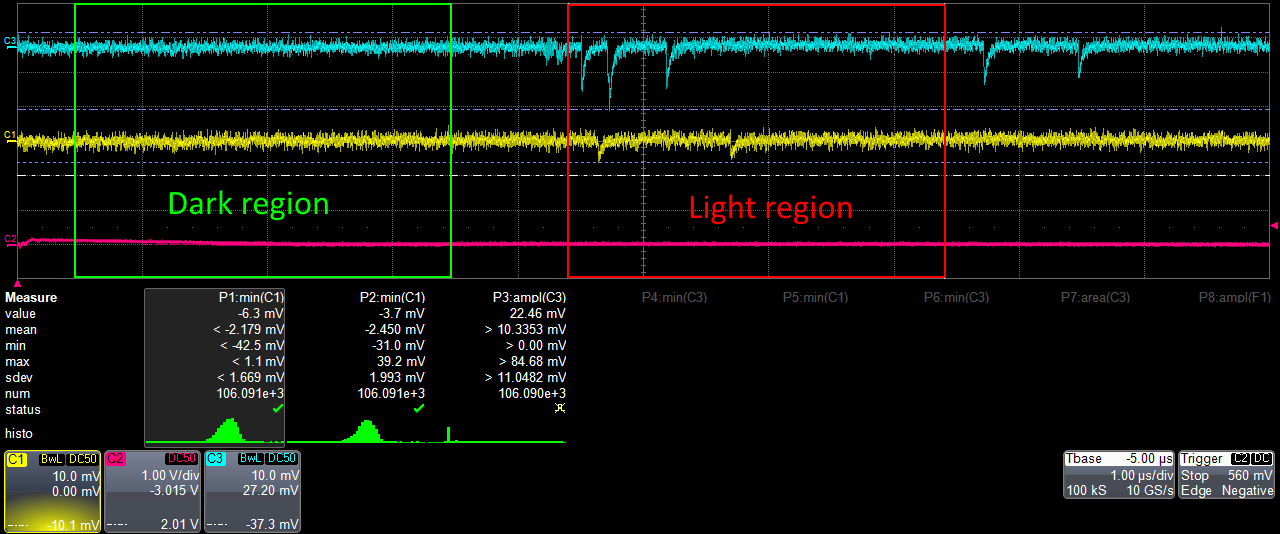
\includegraphics[totalheight=0.22\textwidth,trim=0cm 6.5cm 0cm 0cm, clip=true]{Pictures/blabla/light_region_3.png}
  \centering{\caption{Dark and light regions.}}
  \label{fig:dark_light_region}
  \end{figure}
  
  This error bar are quiet small (appendix for caculation). 
  
  \subsection{analyse : pont entre méthodoligie et solution }
  
  We would like to count the number of time we see a pulse corresponding to one PE peak. One PE peak match with detection of a photon firing 
  severals pixel and triggering an avalanches or show  DN. So in the light region it is not possible to make he difference between a pulse 
  from the detection of a photon or from DN. One way to take in account the pulse of DN is to use the dark region of the scope/waveform. 
  In that region we know for shure that one PE pulse comes obviously from DN.\\
  Considering the fact that DN in the light region or in the dark region appears at the same rate \footnte{follow poisson distribution,
  see appendix}, a solution will be to integrate the zero pe peak of the light and dark region. That's why our formula.
  
  It is obviously  clear that our results for  the PE stuff are not reproductible at all and this for lots reasons.
  
  \subsection{Influence of factors on PE stuff, issues}
  
  Three parameters could influence our results in the ``same'' experimental tets.
  
  \paragraph{the light}
  
  The volatge applied on the falsh lamp increase or decrease the light reaching the detectors. Also the position of the light (far or close of 
  the detector) has an influence. Speak about photon in N2? 
  The voltage of the lamp and the position on the lamp was set. 
  
  \paragraphe{the alignemeent} 
  
  The alignement of the detector with the lamp has an influence on the PE. We noticed the detector of the top wasn't properly aligned with the 
  one of the bottom. 
  
  picture with hole of 1mm. 
  
  \paragraph{the quantity of N2}
  
  The photon can propagate on a distance of mm  in oxygen but on a distance of in N2. That's why we used N2. 
  
  \paragraph{the tempearature}
  
  Th efficiency depend on temperature since Dn depend on temperature \footnote{see section}. 
  The tempearture seem to have an effect on Bs. All the box is cooling. the consequence is that the detector of the top is moving. 
  
  At room temperature, the PE of the Top detector is not constant. the tempearture of the lamp change of 2 degree when the lamp is working. 
  Even is after stabilisation.
  
  
  
  \subsection{further solutions}
  alignement of the lamp. all the box in plastic. Isolate the lamp to avoid radio leak. N2 near the detector. 
  effect of the dust on detecor right bu effect iwth light ? 
  
  
  \chapter{synthèse de l'avancement du proet}


  \chapter{Professional evaluation/Professionla statement}
  
  This internship was really benefit for me. I asked my co-workers 
  lots of questions because they had already worked on that project in the past. 
  I put my theoritical knowledges of matter physics and of detectors physics in pratics during 
  this internship. 
  \\
  
  I have also delighted to my skills learned in differents courses : 
  electronics, analysize and synthesis, research. This internship was 
  a real opportunity to increase my work, with more rigourus and with more method. 
  \\
  
  I was als happier to see that our work had a real impact on. I could saw that/ 
  I was able to see that my work was important for the advancement of the global project. 
  
  \chapter{Human evaluation/Human statement}
  
  From the beginning of my internship I tried to do my best to finish our project on time. 
  The goal was to publish something about my (our) work. This was a real motivation. 
  \\
  
  Also fro the beginning I real enjoyed working with my team. I can confirm that
  discussion moin formel. 
  \\
  
  Finally I really enjoyed my stay in Canada and espcially hiking, speaking english
 discover another culure at work or at home. 
 
 \chapter{conclusion 1 et recommandations}
  
  \\
  
  
 

%%%%%%%%%%%%%%%%%%%%%%%%%%%%%%%%%%%%%%%%%%%%%%%%%%%%%%%%%%%%
%                   bibliography                           %
%%%%%%%%%%%%%%%%%%%%%%%%%%%%%%%%%%%%%%%%%%%%%%%%%%%%%%%%%%%%
\begin{thebibliography}{999}
 \bibitem{ref:wikipedia_beta} Double beta decay, \url{http://en.wikipedia.org/wiki/Double_beta_decay}.
 \bibitem{ref:beta_decay} Double beta decay, \url{http://www2.warwick.ac.uk/study/csde/gsp/eportfolio/directory/crs/phsgbu/research/phdresearch/theory/betadecay/double/}.
 \bibitem{ref:SiPM} Characterisation studies of silicon photomultipliers, {\em LATEX}, 2010, available at \url{http://arxiv.org/abs/1003.6071}.
 \bibitem{ref:DN} Dark Current in Silicon Photomultiplier Pixels: Data and Model, {\em LATEX}, 2012, available at \url{http://www.researchgate.net/publication/258656356_Dark_Current_in_Silicon_Photomultiplier_Pixels_Data_and_Model}.
 \bibitem{ref:CT} Modeling crosstalk in silicon photomultipliers, {\em LATEX}, 2013, available at \url{http://arxiv.org/abs/1302.1455}.
 \bibitem{ref:nEXO} Characterization of Silicon Photomultipliers for nEXO, {\em LATEX}, 2013, available at \url{http://arxiv.org/abs/1502.07837}. 
\end{thebibliography}

\end{document}
  

